\documentclass[11pt,a4paper,openany]{book}
\usepackage[utf8]{inputenc}
\usepackage[T1]{fontenc}
\usepackage[spanish,es-tabla]{babel}
\usepackage{lmodern}
\usepackage[top=2.5cm,bottom=2.5cm,left=2.5cm,right=2.5cm,headheight=14pt]{geometry}
\usepackage{microtype}
\usepackage[table,xcdraw]{xcolor}
\definecolor{headerblue}{RGB}{24,43,73}
\definecolor{accentblue}{RGB}{30,80,150}
\definecolor{lightbg}{RGB}{248,249,251}
\definecolor{bordergray}{RGB}{220,224,230}
\usepackage{amsmath,amssymb,amsthm}
\usepackage{graphicx}
\graphicspath{{assets/originales/}{../public/assets/}{./}}
\usepackage{hyperref}
\hypersetup{colorlinks=true,linkcolor=accentblue,citecolor=accentblue,urlcolor=accentblue,pdftitle={LogiLearn -- Manual de Usuario},pdfauthor={UNPRG MATG1001},bookmarksnumbered=true,breaklinks=true}
\usepackage{booktabs,tabularx,array,longtable,enumitem,caption,float}
\usepackage{fancyhdr}
\pagestyle{fancy}
\fancyhf{}
\renewcommand{\headrulewidth}{0.4pt}
\fancyhead[LE,RO]{\small\textsc{LogiLearn -- Manual de Usuario}}
\fancyhead[RE,LO]{\small\leftmark}
\fancyfoot[C]{\small\thepage}
\fancypagestyle{plain}{\fancyhf{}\fancyfoot[C]{\small\thepage}\renewcommand{\headrulewidth}{0pt}}
\usepackage{titlesec}
\titleformat{\chapter}[display]{\Huge\bfseries\color{headerblue}}{\chaptername\ \thechapter}{12pt}{\Huge}
\titleformat{\section}{\Large\bfseries\color{headerblue}}{}{0pt}{}
\titleformat{\subsection}{\large\bfseries\color{accentblue}}{}{0pt}{}
\usepackage{listings}
\lstdefinelanguage{TypeScript}{keywords={const,let,function,return,import,export,for,if,else,new},keywordstyle=\color{accentblue}\bfseries,comment=[l]{//},commentstyle=\color{gray}\itshape,sensitive=true}
\lstset{basicstyle=\ttfamily\footnotesize,breaklines=true,frame=single,rulecolor=\color{bordergray},numbers=left,numberstyle=\tiny\color{gray},showstringspaces=false,tabsize=2,extendedchars=true,literate={á}{{\'a}}1 {é}{{\'e}}1 {í}{{\'i}}1 {ó}{{\'o}}1 {ú}{{\'u}}1 {ñ}{{\~n}}1}
\begin{document}
\frontmatter
\begin{titlepage}
\centering
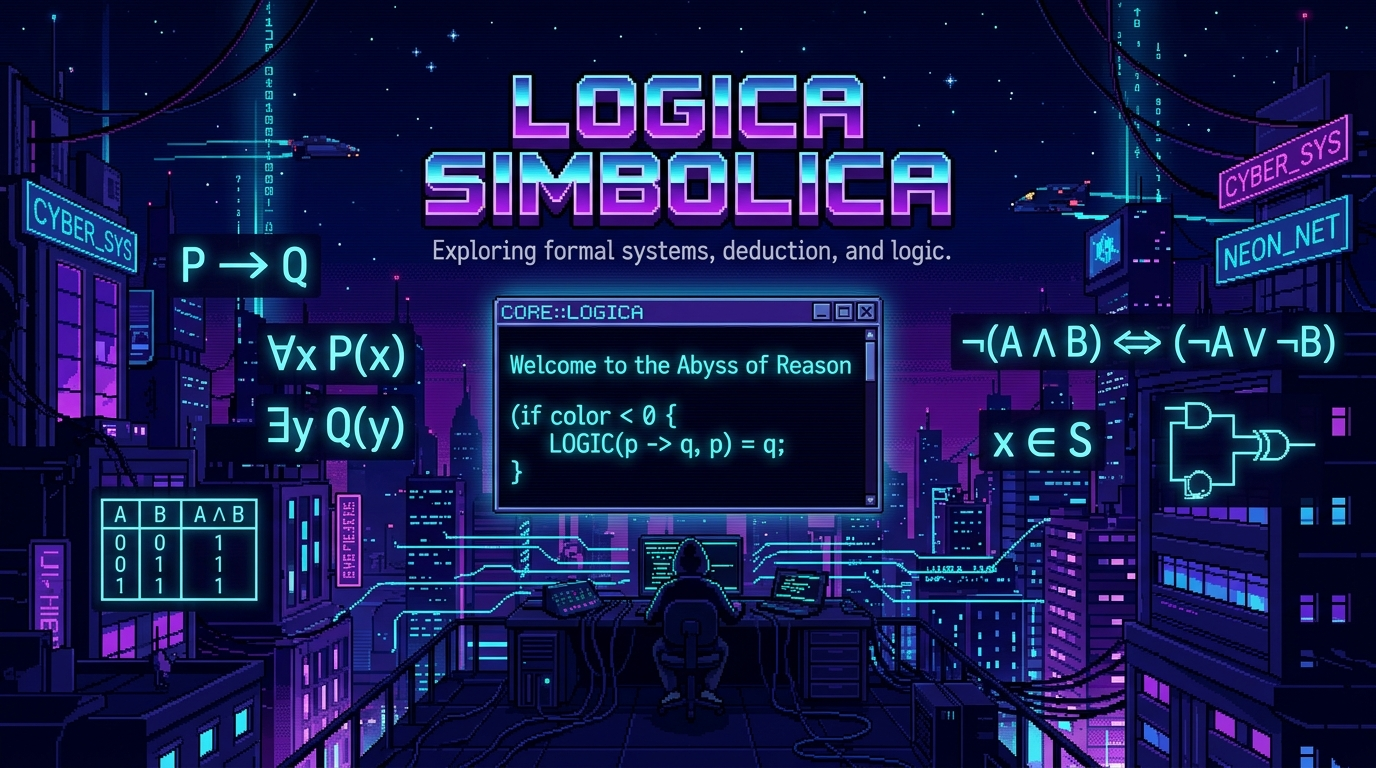
\includegraphics[width=0.55\textwidth]{public_banner.jpg}\par
\vspace{0.6cm}
{\Large Universidad Nacional Pedro Ruiz Gallo\par}
{\large Facultad de Ingenier\'ia Civil, de Sistemas y de Arquitectura\par}
{\large Escuela Profesional de Ingenier\'ia de Sistemas\par}
\vspace{0.9cm}
{\Huge \bfseries\color{headerblue} LogiLearn\par}
{\LARGE L\'ogica Simb\'olica Global\par}
\vspace{0.3cm}
{\large \textbf{Manual de Usuario Unificado}\par}
{\large Plataforma web interactiva --- 4 m\'odulos, 4 equipos, 100\% s\'ilabo MATG1001\par}
\vspace{0.8cm}
\begin{center}
\begin{tabular}{ll}
\toprule
\textbf{Curso:} & MATG1001 --- 2026 I, II Ciclo (3 cr\'editos) \\
\textbf{Docente:} & Dr. Mardo Victor Gonzales Herrera \\
\textbf{L\'ider:} & Enrique D\'iaz Cayaca \\
\textbf{Equipos:} & Sinergia (Tablas) $\cdot$ Hijos de Linus (Inferencias) \\
& Modus Innova (Cuantificadores) $\cdot$ Linus (Conjuntos) \\
\textbf{Versi\'on:} & 3.5 --- Septiembre 2026 \\
\textbf{Repositorio:} & \url{https://github.com/EnriDiazCayaca/logica_simbolica_global} \\
\bottomrule
\end{tabular}
\end{center}
\vspace{0.8cm}
{\small Lambayeque, Per\'u --- Septiembre 2026\par}
\end{titlepage}
\tableofcontents
\listoffigures
\listoftables
\mainmatter

\chapter{Introducci\'on general}
\label{ch:intro}
\section{Qu\'e es LogiLearn?}
LogiLearn es una plataforma web colaborativa, gratuita y de c\'odigo abierto donde cada tema del s\'ilabo de L\'ogica Simb\'olica (MATG1001) es un motor verificable. A diferencia de un apunte est\'atico, cada m\'odulo eval\'ua f\'ormulas reales: genera tablas de verdad, valida inferencias, eval\'ua cuantificadores sobre dominios finitos y opera conjuntos con diagramas de Venn interactivos. El proyecto fue construido por el aula del curso 2026 I, organizado en cuatro equipos de dominio, cada uno responsable de un m\'odulo.

\begin{table}[H]
\centering
\caption{Mapa de m\'odulos y equipos responsables}
\label{tab:modulos}
\begin{tabular}{lll}
\toprule
M\'odulo & Ruta & Equipo \\
\midrule
Tablas de Verdad & \texttt{/tablas} & Sinergia \\
Inferencias L\'ogicas & \texttt{/inferencias} & Hijos de Linus \\
Cuantificadores & \texttt{/cuantificadores} & Modus Innova \\
Conjuntos y Venn & \texttt{/conjuntos} & Linus \\
Aprender (transversal) & \texttt{/aprender} & Compartido \\
Leyes L\'ogicas (transversal) & \texttt{/leyes-logicas} & Compartido \\
\bottomrule
\end{tabular}
\end{table}

\section{A qui\'en va dirigido este manual}
Este manual est\'a dirigido a estudiantes del curso y al docente. No requiere conocimientos de programaci\'on ni de Git. Cada cap\'itulo es autocontenido: indica requisitos, describe la interfaz paso a paso con capturas, propone ejemplos resueltos y cierra con soluci\'on de problemas. La terminolog\'ia se unifica en todo el documento: $D \subset \mathbb{Z}$ denota siempre un dominio finito de n\'umeros enteros; $V$ y $F$ denotan verdadero y falso; los conectivos se escriben $\lnot$, $\land$, $\lor$, $\to$, $\leftrightarrow$; los cuantificadores $\forall$ (para todo) y $\exists$ (existe).

\section{Convenciones de lectura}
Los nombres de botones aparecen en \textbf{negrita} (por ejemplo, \textbf{Generar tabla}). Las f\'ormulas aparecen en modo matem\'atico (por ejemplo, $P \land Q \to R$). Las rutas de la aplicaci\'on aparecen en \texttt{monoespaciado} (por ejemplo, \texttt{/tablas}). Las figuras llevan pie numerado y se referencian en el texto (por ejemplo, la Figura~\ref{fig:banner} muestra el banner institucional).

\begin{figure}[H]
\centering
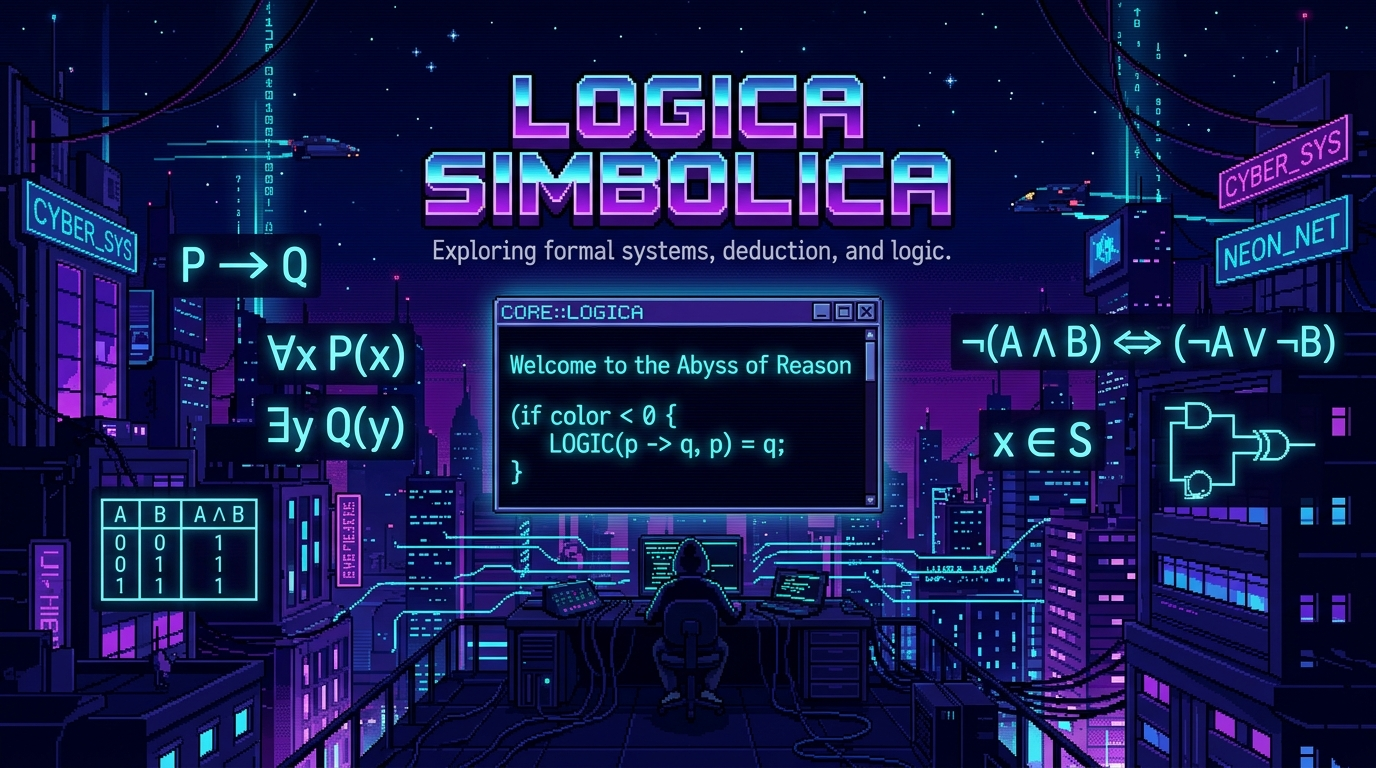
\includegraphics[width=0.9\textwidth]{public_banner.jpg}
\caption{Banner institucional de la plataforma LogiLearn}
\label{fig:banner}
\end{figure}

\section{Estructura del manual}
El Cap\'itulo~\ref{ch:acceso} describe instalaci\'on y acceso. Los Cap\'itulos~\ref{ch:tablas} a~\ref{ch:cuantificadores} cubren los cuatro m\'odulos de dominio, cada uno con teor\'ia m\'inima, interfaz paso a paso, ejemplos y errores frecuentes. El Cap\'itulo~\ref{ch:transversales} cubre los m\'odulos transversales. Los ap\'endices re\'unen la galer\'ia de evidencias, el glosario y la bibliograf\'ia.

\chapter{Acceso e instalaci\'on}
\label{ch:acceso}
\section{Requisitos}
Un navegador moderno (Chrome, Firefox, Edge o Safari) actualizado, conexi\'on a internet y una resoluci\'on m\'inima de 360 p\'ixeles de ancho. No se requiere instalar complementos. Para desarrollo local se requiere Node.js 18 o superior.

\section{Uso sin instalaci\'on (recomendado para estudiantes)}
La forma recomendada es usar la versi\'on publicada en GitHub Pages. Basta abrir la URL de producci\'on en el navegador. Cada Pull Request genera adem\'as una vista previa temporal en Netlify con URL \'unica, \'util para revisar cambios antes de publicarlos.

\section{Instalaci\'on local paso a paso}
\begin{enumerate}[leftmargin=*]
\item Clonar el repositorio con \texttt{git clone} desde la URL del proyecto.
\item Instalar dependencias con \texttt{npm install}.
\item Iniciar el servidor con \texttt{npm run dev} y abrir \url{http://localhost:5173}.
\item Verificar la compilaci\'on con \texttt{npm run build}.
\item Ejecutar las pruebas con \texttt{npm test} (17 archivos, 189 pruebas).
\end{enumerate}

\section{Navegaci\'on global}
La barra superior muestra el logo y seis enlaces: Inicio, Aprender, Tablas de verdad, Leyes l\'ogicas, Ejercicios y Progreso. Los m\'odulos de Cuantificadores, Conjuntos e Inferencias se alcanzan desde las tarjetas de la p\'agina de inicio. El pie de p\'agina indica el proyecto de aula 2026 y la universidad.

\section{Problemas de acceso}
Si la p\'agina publicada muestra contenido antiguo, realice una recarga forzada (Ctrl + Shift + R). Si el servidor local no arranca, verifique que el puerto 5173 est\'e libre y que las dependencias est\'en instaladas. Si una vista previa de Netlify no carga, compruebe que el Pull Request asociado siga abierto.

\chapter{Tablas de verdad (Equipo Sinergia)}
\label{ch:tablas}
\section{Qu\'e hace este m\'odulo}
El m\'odulo de Tablas de Verdad genera la tabla completa de una f\'ormula proposicional, clasifica el resultado como tautolog\'ia, contradicci\'on o contingencia, y explica c\'omo se obtuvo cada valor. Implementa un motor proposicional con precedencia $\lnot > \land > \lor > \to > \leftrightarrow$.

\begin{table}[H]
\centering
\caption{Los cinco conectivos del motor}
\label{tab:conectivos}
\begin{tabular}{lll}
\toprule
Conectivo & S\'imbolo & Lectura \\
\midrule
Negaci\'on & $\lnot$ & no $p$ \\
Conjunci\'on & $\land$ & $p$ y $q$ \\
Disyunci\'on & $\lor$ & $p$ o $q$ \\
Condicional & $\to$ & si $p$ entonces $q$ \\
Bicondicional & $\leftrightarrow$ & $p$ si y solo si $q$ \\
\bottomrule
\end{tabular}
\end{table}

\section{Interfaz paso a paso}
\begin{enumerate}[leftmargin=*]
\item \textbf{Cabecera.} El t\'itulo \textit{Tablas de Verdad} y el subt\'itulo \textit{Analiza y eval\'ua proposiciones mediante tablas de verdad} identifican el m\'odulo.
\item \textbf{Entrada.} La etiqueta \textit{Ingresa una f\'ormula l\'ogica} acompa\~na al campo de texto con ejemplo $P \land Q \to R$. El bot\'on \textbf{Crear tabla de verdad} genera la tabla; tambi\'en funciona la tecla Enter.
\item \textbf{Conectores l\'ogicos.} Cinco botones con s\'imbolo y etiqueta (AND, OR, NOT, IMPL, BICOND). Al pulsarlos insertan $\land$, $\lor$, $\lnot$, $\to$, $\leftrightarrow$ en la entrada. La Figura~\ref{fig:sin-gramatica} muestra la gram\'atica que reconoce el motor.
\item \textbf{Variables proposicionales.} El panel \textit{Variables proposicionales} lista cada variable detectada ($P$, $Q$, $R$) con un interruptor. Desactivar una variable la excluye de la tabla, \'util para reducir combinaciones.
\item \textbf{Clasificaci\'on l\'ogica.} El panel muestra \textit{TAUTOLOG\'IA} (todo $V$, fondo verde), \textit{CONTRADICCI\'ON} (todo $F$, fondo rojo) o \textit{CONTINGENCIA} (mixto, \'ambar), con explicaci\'on y conteo de combinaciones verdaderas sobre el total.
\item \textbf{Tabla.} Columnas para variables, subexpresiones intermedias y Resultado ($V$/$F$ en verde/rojo). En pantallas peque\~nas la tabla se desplaza horizontalmente.
\item \textbf{Explicaci\'on.} La secci\'on \textit{\'Como se obtuvo el resultado?} lista cada subexpresi\'on evaluada. El bot\'on \textit{Ver resoluci\'on paso a paso} despliega el detalle por precedencia.
\end{enumerate}

\begin{figure}[H]
\centering

\includegraphics[width=0.9\textwidth]{informe_scratch_sinergia_p04_1142x235_778970ea.png}
\caption{Gram\'atica del motor proposicional (material original del equipo Sinergia)}
\label{fig:sin-gramatica}
\end{figure}

\begin{figure}[H]
\centering

\includegraphics[width=0.9\textwidth]{informe_scratch_sinergia_p07_1142x607_eb18271a.png}
\caption{Tokenizador y normalizaci\'on de notaciones (material original del equipo Sinergia)}
\label{fig:sin-token}
\end{figure}

\begin{figure}[H]
\centering

\includegraphics[width=0.9\textwidth]{informe_scratch_sinergia_p08_1142x633_f4c6524a.png}
\caption{Analizador sint\'actico descendente recursivo (material original del equipo Sinergia)}
\label{fig:sin-parser}
\end{figure}

\section{Ejemplos resueltos}
\textbf{Ejemplo 1.} $P \lor \lnot P$ produce una \textit{TAUTOLOG\'IA}: con una variable hay 2 filas y ambas dan $V$. \textbf{Ejemplo 2.} $P \land \lnot P$ produce una \textit{CONTRADICCI\'ON}: ambas filas dan $F$. \textbf{Ejemplo 3.} $P \to Q$ produce una \textit{CONTINGENCIA}: de 4 filas, 3 dan $V$ y 1 da $F$ (cuando $P$ es $V$ y $Q$ es $F$). \textbf{Ejemplo 4.} $(P \land Q) \to R$ con tres variables genera $2^{3} = 8$ filas; la Figura~\ref{fig:sin-eval} ilustra la evaluaci\'on por subexpresiones.

\begin{figure}[H]
\centering

\includegraphics[width=0.9\textwidth]{informe_scratch_sinergia_p12_1143x951_ec5d5c9c.png}
\caption{Evaluaci\'on sem\'antica y generaci\'on de filas (material original del equipo Sinergia)}
\label{fig:sin-eval}
\end{figure}

\section{Errores frecuentes}
Si la tabla queda vac\'ia, pulse \textbf{Crear tabla de verdad}. Si aparece error de sintaxis, revise par\'entesis y escriba variables en may\'usculas ($P$, $Q$, $R$). Si la clasificaci\'on no aparece, verifique que al menos una variable est\'e activa. Recuerde que la implicaci\'on $P \to Q$ solo es $F$ cuando el antecedente es $V$ y el consecuente es $F$.

\chapter{Conjuntos y diagramas de Venn (Equipo Linus)}
\label{ch:conjuntos}
\section{Qu\'e hace este m\'odulo}
El m\'odulo de Conjuntos es una calculadora interactiva de operaciones b\'asicas y de familias de conjuntos, con diagramas de Venn que muestran regiones exactas y un modo para conjuntos disjuntos.

\begin{table}[H]
\centering
\caption{Operaciones disponibles}
\label{tab:conjuntos-ops}
\begin{tabular}{ll}
\toprule
Operaci\'on & Lectura \\
\midrule
$A \cup B$ & Uni\'on \\
$A \cap B$ & Intersecci\'on \\
$A \setminus B$ & Diferencia $A$ menos $B$ \\
$B \setminus A$ & Diferencia $B$ menos $A$ \\
$A^{c}$ & Complemento de $A$ \\
$P(A)$ & Conjunto potencia de $A$ \\
\bottomrule
\end{tabular}
\end{table}

\section{Uso paso a paso}
La cabecera \textit{Teor\'ia de Conjuntos y Diagramas de Venn} identifica el m\'odulo. Defina el Universo $U$ y los conjuntos $A$ y $B$ con listas separadas por comas (por ejemplo, \texttt{1, 2, 3, 4}). Seleccione una operaci\'on; para la potencia elija adem\'as el conjunto base ($P(A)$, $P(B)$, $P(A \cup B)$, etc.). El diagrama SVG de $400 \times 270$ colorea cada regi\'on seg\'un la operaci\'on. El resultado aparece en notaci\'on $\{ \}$ monoespaciada con el total $2^{n}$ de subconjuntos cuando corresponde. El panel de propiedades indica $A \subseteq B$, $B \subseteq A$, $A = B$ y Disjuntos con insignias S\'i/No. El verificador de pertenencia responde $\in$ o $\notin$ para $A$, $B$ y $U$.

\begin{figure}[H]
\centering
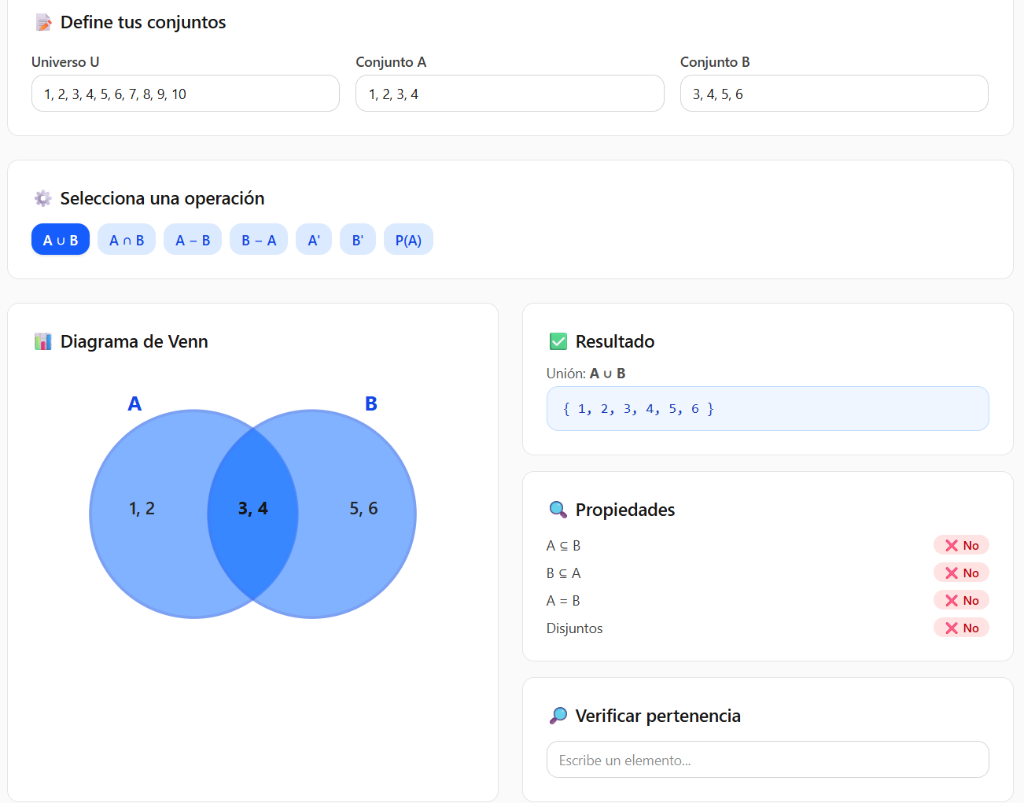
\includegraphics[width=0.85\textwidth]{informe_scratch_linus_p03_1024x803_e056eaf0.png}
\caption{Boceto inicial del m\'odulo de conjuntos (material original del equipo Linus)}
\label{fig:lin-wire}
\end{figure}

\begin{figure}[H]
\centering
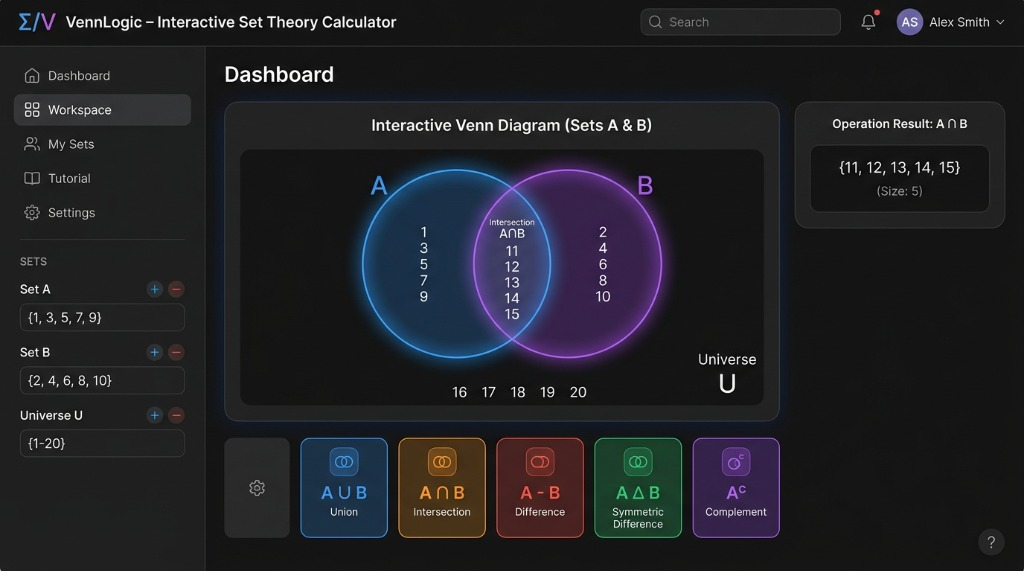
\includegraphics[width=0.9\textwidth]{informe_scratch_linus_p06_1024x571_23455df9.jpeg}
\caption{Diagrama de Venn interactivo (material original del equipo Linus)}
\label{fig:lin-venn}
\end{figure}

\section{Conjunto potencia}
Si el conjunto base tiene m\'as de 10 elementos, la aplicaci\'on muestra una advertencia con el total $2^{n}$ en lugar de listar todos los subconjuntos, pues el crecimiento es exponencial. En caso contrario lista $\{ \emptyset, \{1\}, \ldots \}$.

\begin{figure}[H]
\centering
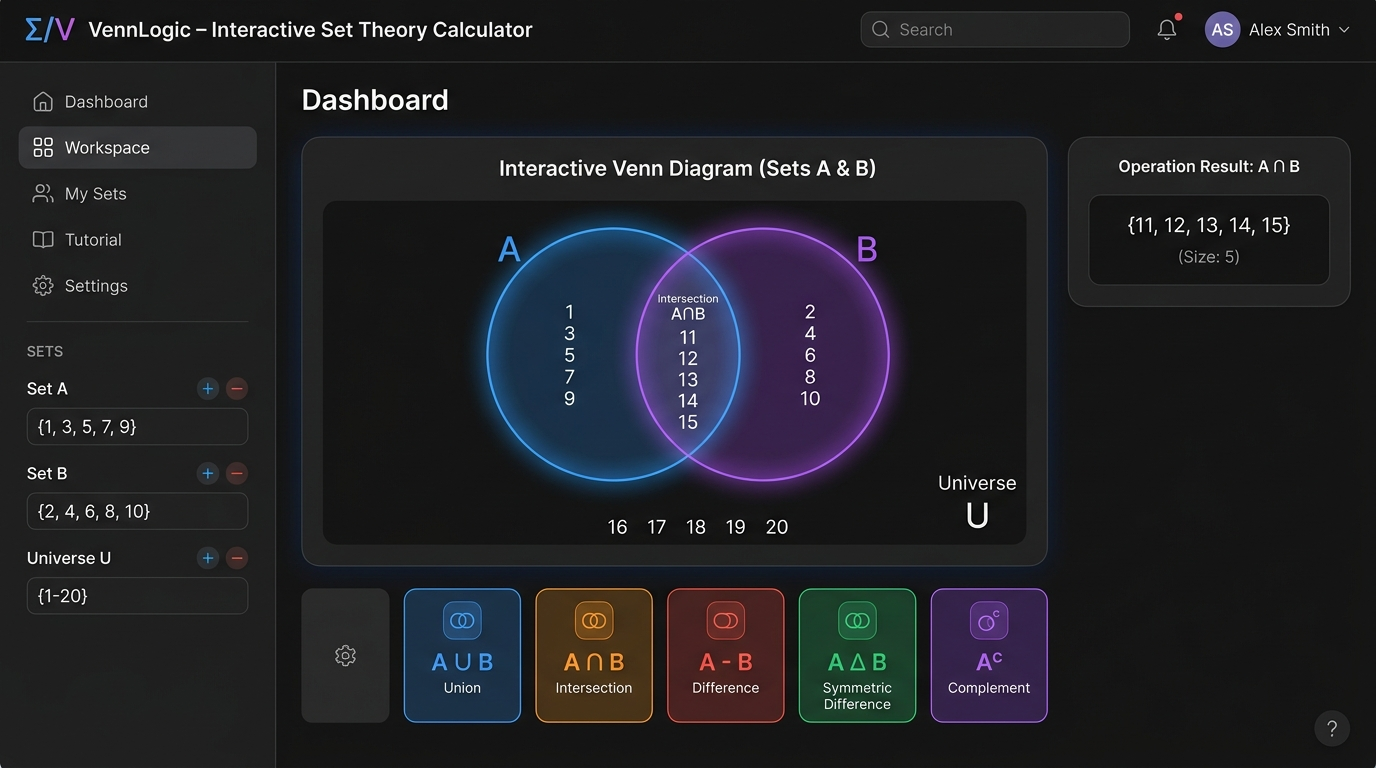
\includegraphics[width=0.48\textwidth]{propuesta_linus_propuesta-jordy.jpg}
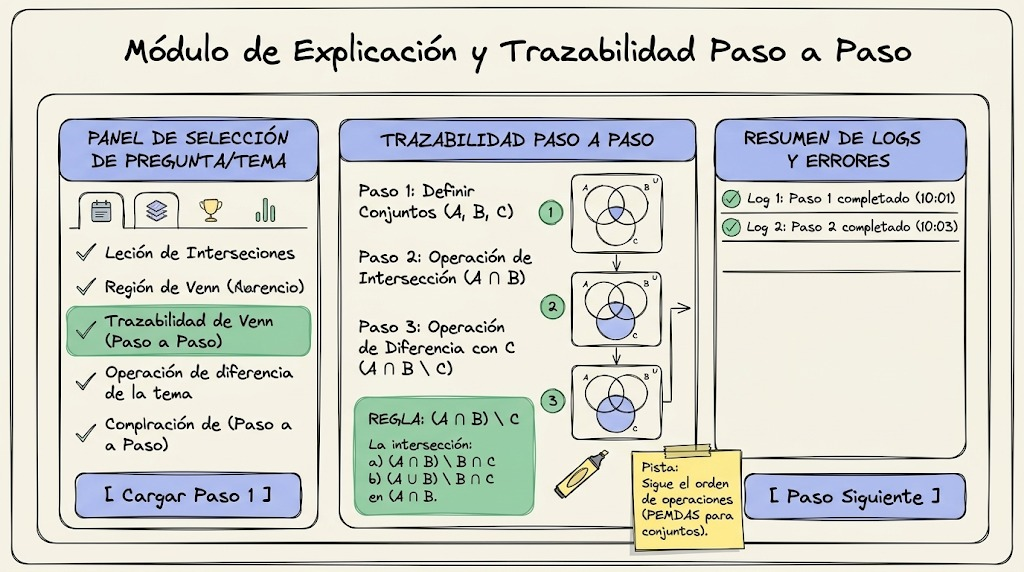
\includegraphics[width=0.48\textwidth]{propuesta_linus_propuesta-alejandro.jpg}
\caption{Bocetos iniciales del equipo Linus (archivos originales de propuesta)}
\label{fig:lin-bocetos}
\end{figure}

\section{Ejemplos y errores}
Con $U = \{1, \ldots, 10\}$, $A = \{1,2,3,4\}$, $B = \{3,4,5,6\}$ la uni\'on da $\{1,2,3,4,5,6\}$ y la intersecci\'on $\{3,4\}$. Si el diagrama aparece vac\'io, defina primero $U$ y luego $A$ y $B$. Si la potencia no se calcula, reduzca el conjunto base.

\chapter{Inferencias l\'ogicas (Equipo Hijos de Linus)}
\label{ch:inferencias}
\section{Qu\'e hace este m\'odulo}
El m\'odulo valida si una conclusi\'on se deduce de unas premisas con 11 reglas de inferencia, muestra la trazabilidad paso a paso y, si el argumento es inv\'alido, exhibe el contraejemplo. Incluye \'arbol sint\'actico y traducci\'on a lenguaje natural.

\begin{table}[H]
\centering
\caption{Reglas de inferencia soportadas (selecci\'on)}
\label{tab:reglas}
\begin{tabular}{ll}
\toprule
Regla & Esquema \\
\midrule
Modus Ponens & $p, \; p \to q \vdash q$ \\
Modus Tollens & $\lnot q, \; p \to q \vdash \lnot p$ \\
Silogismo Hipot\'etico & $p \to q, \; q \to r \vdash p \to r$ \\
Silogismo Disyuntivo & $p \lor q, \; \lnot p \vdash q$ \\
Adici\'on & $p \vdash p \lor q$ \\
Simplificaci\'on & $p \land q \vdash p$ \\
\bottomrule
\end{tabular}
\end{table}

\section{Pesta\~nas}
\textbf{Simbolog\'ia Formal} es la pesta\~na por defecto (t\'itulo \textit{Explorador de Inferencias L\'ogicas}). \textbf{Lenguaje Natural} traduce s\'imbolos a espa\~nol con un mapa como $p \mapsto$ ``Llueve''. \textbf{\'Arbol Sint\'actico} dibuja la estructura jer\'arquica con zoom.

\section{Flujo de uso}
\begin{enumerate}[leftmargin=*]
\item Escriba premisas numeradas y conclusi\'on (por ejemplo, $P \to Q$, $P \vdash Q$).
\item Pulse \textbf{Demostrar}. El indicador muestra \textit{V\'alida}, \textit{Inv\'alida} o \textit{V\'alida (Ind.)}.
\item Lea la trazabilidad: cada paso cita sus l\'ineas base y la regla aplicada. Exporte a \LaTeX\ o Markdown en un clic.
\item Consulte el historial local de 6 ejercicios recientes con el bot\'on \textit{Historial}.
\end{enumerate}

\begin{figure}[H]
\centering
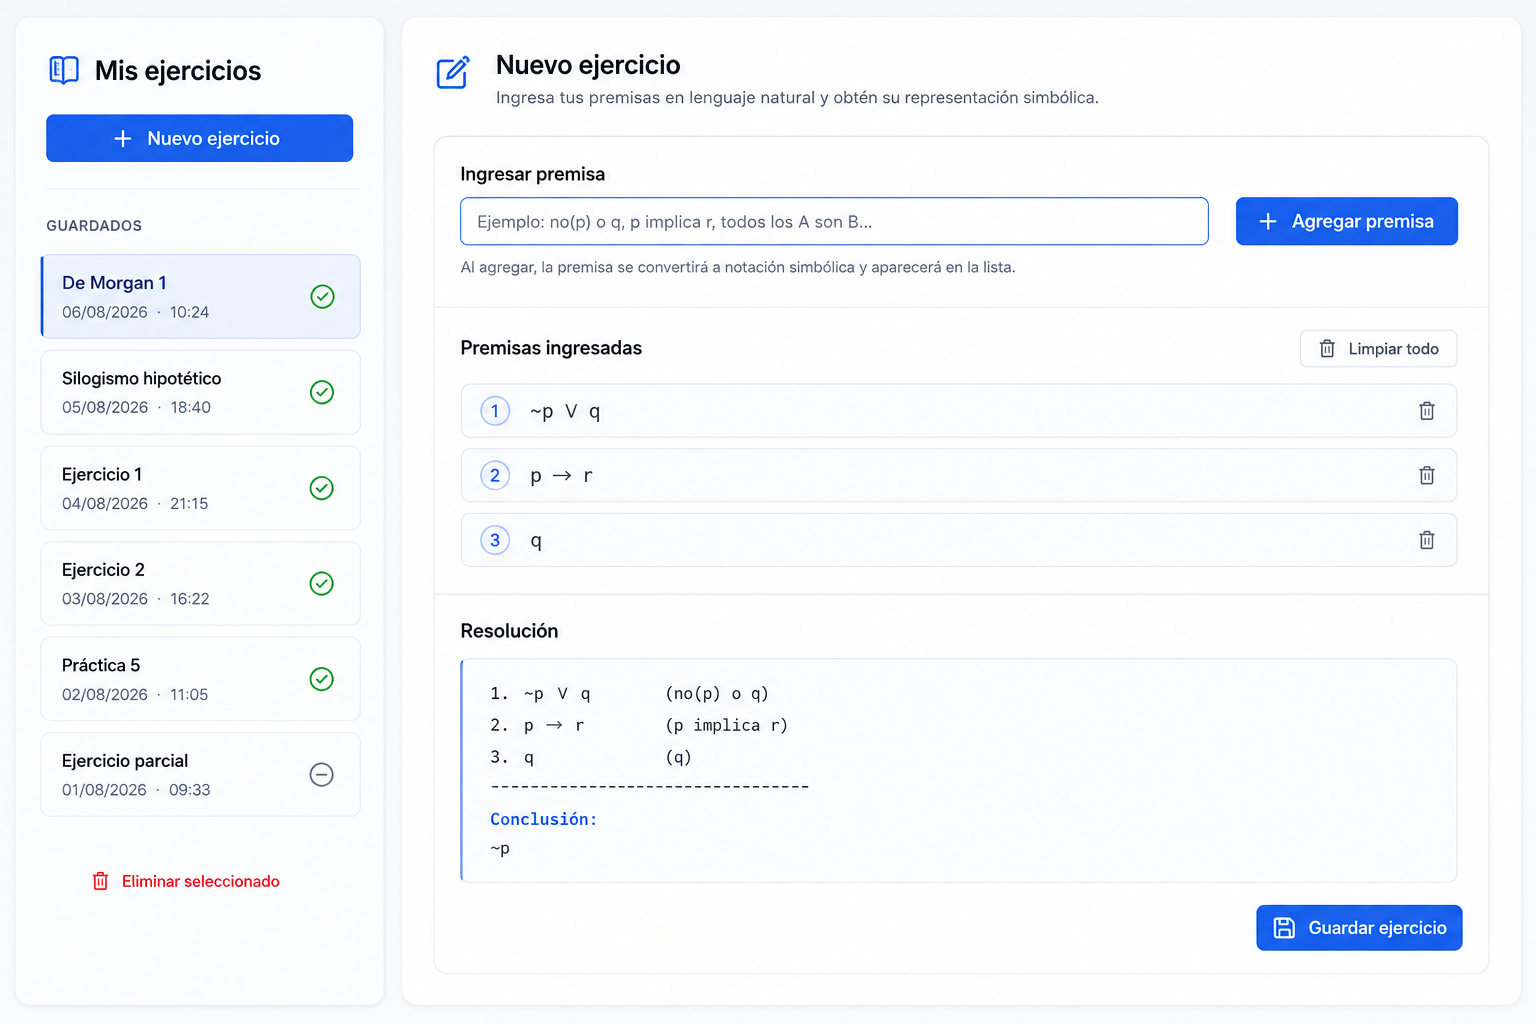
\includegraphics[width=0.85\textwidth]{propuesta_hijos_propuesta-alex.png}
\caption{Boceto del \'arbol sint\'actico (archivo original del equipo Hijos de Linus)}
\label{fig:hijos-ast}
\end{figure}

\begin{figure}[H]
\centering
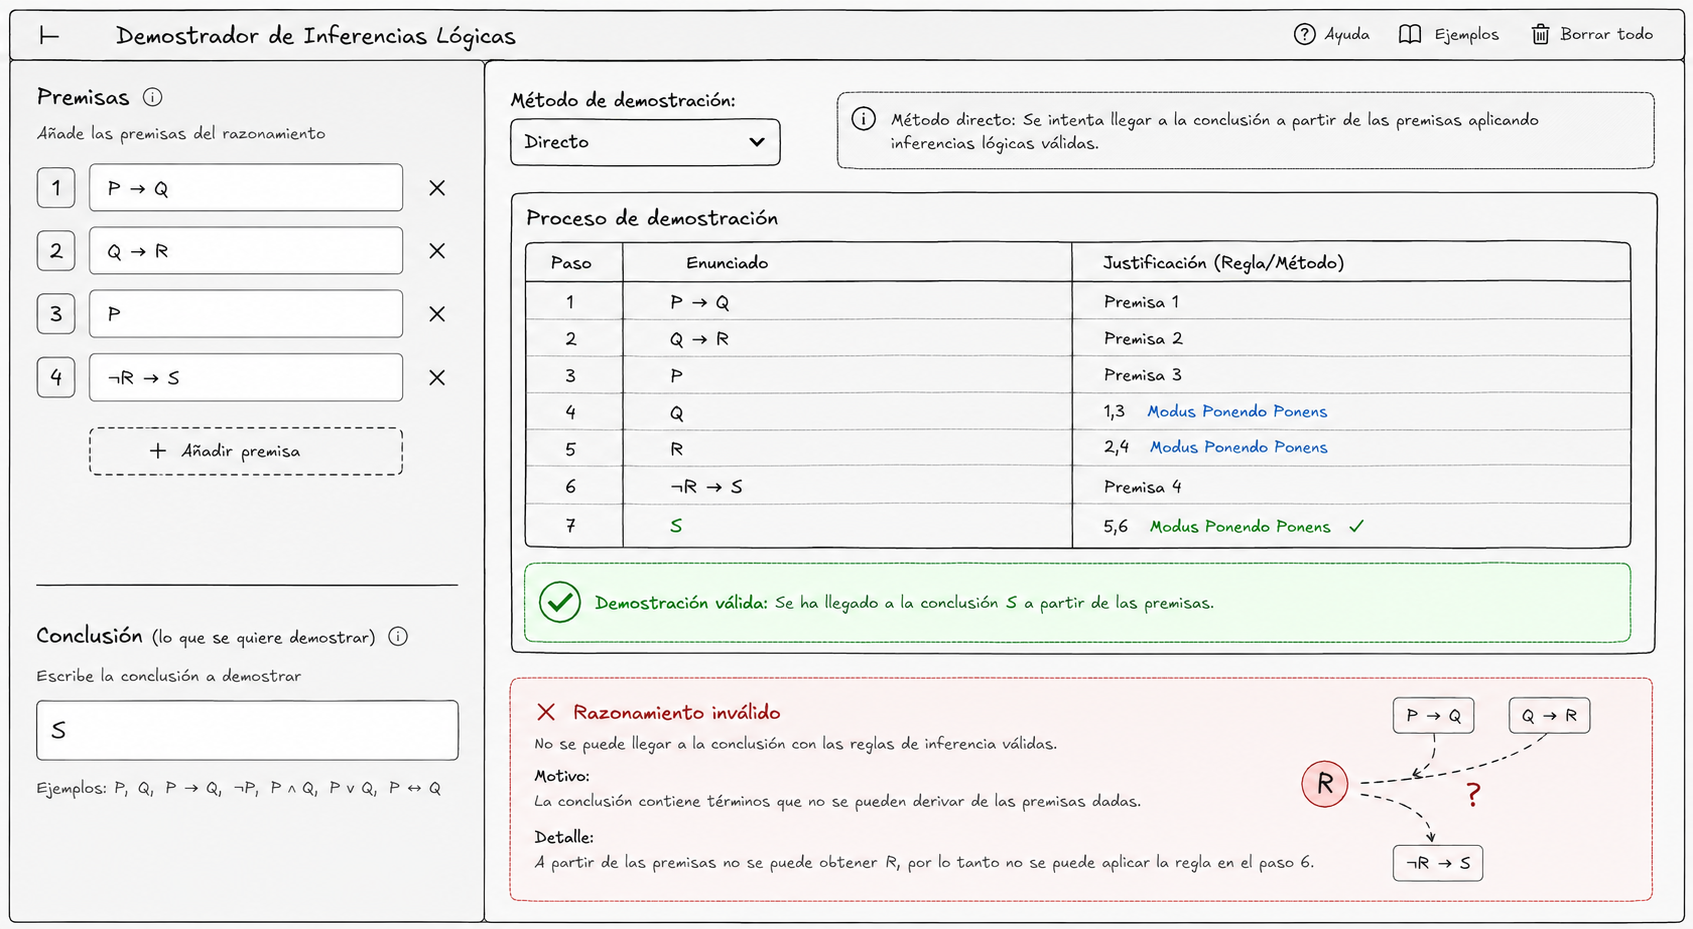
\includegraphics[width=0.85\textwidth]{propuesta_hijos_propuesta-arnold.png}
\caption{Interfaz de c\'alculo y resoluci\'on (archivo original del equipo Hijos de Linus)}
\label{fig:hijos-ui}
\end{figure}

\section{Ejemplo y errores}
$P \to Q$, $P \vdash Q$ es v\'alida por Modus Ponens en una iteraci\'on. $P \to Q$, $Q \vdash P$ es inv\'alida (afirmaci\'on del consecuente) con contraejemplo $P = F$, $Q = V$. Si el sistema marca inv\'alida siempre, revise la numeraci\'on de premisas y use un ejemplo r\'apido.

\chapter{Cuantificadores y leyes (Equipo Modus Innova)}
\label{ch:cuantificadores}
\section{Qu\'e hace este m\'odulo}
Eval\'ua $\forall$ (para todo) y $\exists$ (existe) sobre dominios finitos $D \subset \mathbb{Z}$ y reescribe f\'ormulas de predicados con disyunci\'on fuerte $\Delta$. Las leyes de De Morgan para cuantificadores son $\lnot(\forall x\,P(x)) \equiv \exists x\,\lnot P(x)$ y $\lnot(\exists x\,P(x)) \equiv \forall x\,\lnot P(x)$.

\begin{figure}[H]
\centering
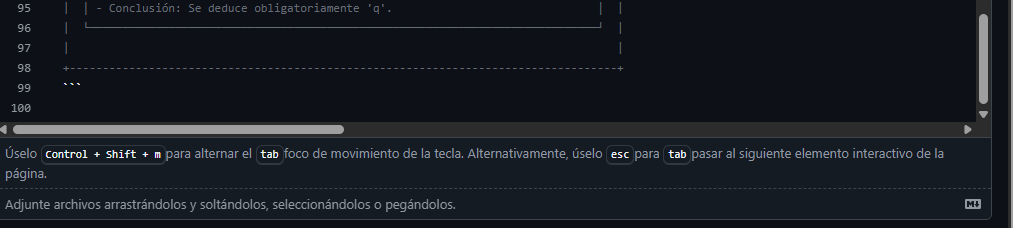
\includegraphics[width=0.9\textwidth]{informe_scratch_modusinnova_p06_1013x228_a2c880e2.png}
\caption{Boceto de QuantifiWeb (material original del equipo Modus Innova)}
\label{fig:mod-boceto}
\end{figure}

\begin{figure}[H]
\centering
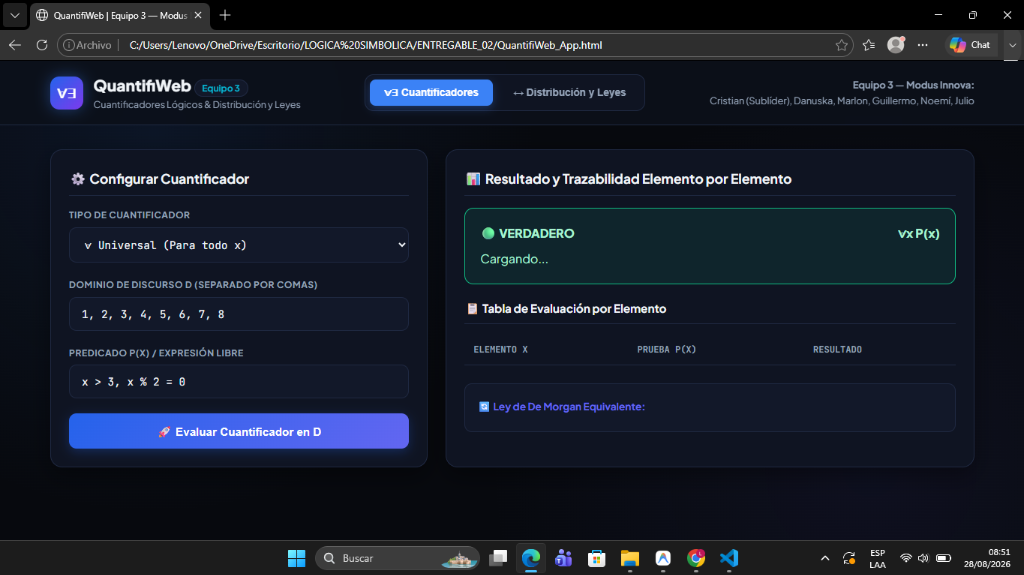
\includegraphics[width=0.9\textwidth]{informe_scratch_modusinnova_p07_1024x575_9d31f7a8.png}
\caption{Motor de cuantificadores (material original del equipo Modus Innova)}
\label{fig:mod-motor}
\end{figure}

\section{Pesta\~na Cuantificadores}
La cabecera \textit{Comprende y aplica los cuantificadores} identifica el m\'odulo. Elija \textit{Para todo} o \textit{Existe}, defina el dominio $D \subset \mathbb{Z}$ como lista (\texttt{1, 2, 3}) o rango ($D = \{x \in \mathbb{Z} : 0 < x < 9\}$) y el predicado $p(x)$ con interruptor \textit{Libre} ($x \% 2 === 0$). Los s\'imbolos r\'apidos $\forall \exists \in \to \land \lor \lnot \equiv \therefore \Delta \oplus$ insertan notaci\'on. Los botones \textit{Evaluar}, \textit{Ejemplo simple} y \textit{Ejemplo rango} ejecutan la evaluaci\'on. El resultado \textit{VERDADERO/FALSO} incluye \textit{Contraejemplo: $(x = 1)$, pues $P(1) = F$} o \textit{Testigo} y la tabla de trazabilidad por elemento.

\begin{figure}[H]
\centering
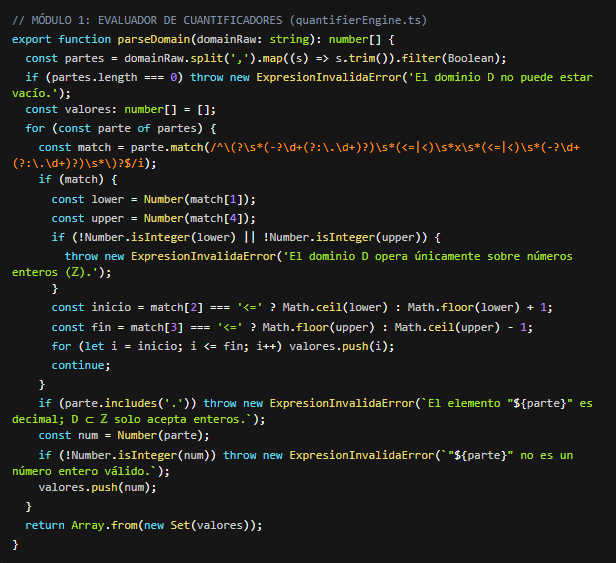
\includegraphics[width=0.9\textwidth]{informe_scratch_modusinnova_p13_616x563_3cb03fed.png}
\caption{Validaci\'on del dominio $D \subset \mathbb{Z}$ (material original del equipo Modus Innova)}
\label{fig:mod-dominio}
\end{figure}

\section{Pesta\~na Distribuci\'on y Leyes}
El resolutor \textit{Resolver Autom\'aticamente} ($\Delta$ soportado) aplica el pipeline \textit{Doble Negaci\'on $\to$ $\Delta$ $\to$ Bicondicional $\to$ Implicaci\'on $\to$ De Morgan $\to$ Distribuci\'on}. Con entrada $\lnot(A \land B) \leftrightarrow C$ produce pasos \textit{Antes/Despu\'es} y \textit{Resultado final}. El cat\'alogo muestra las 12 leyes con buscador.

\section{Ejemplos}
$\forall x \in \{2,4,6\}$ con $x$ par da $V$ sin contraejemplo. $\exists x \in \{1,3,5\}$ con $x \% 2 == 0$ da $F$. El rango $0 < x < 9$ con $x \% 2 == 0$ da $F$ con contraejemplo $x = 1$.

\chapter{M\'odulos transversales}
\label{ch:transversales}
\section{Aprender}
\subsection{Los cinco conectores en detalle}
\begin{table}[H]
\centering
\caption{Conectores con s\'imbolo l\'ogico (nunca la palabra suelta)}
\label{tab:conectores-det}
\begin{tabular}{llll}
\toprule
Conector & S\'imbolo & Ejemplo & Condici\'on de verdad \\
\midrule
Negaci\'on & $\lnot$ & $\lnot p$ & $V$ si $p$ es $F$ \\
Conjunci\'on & $\land$ & $p \land q$ & $V$ solo si ambas son $V$ \\
Disyunci\'on & $\lor$ & $p \lor q$ & $F$ solo si ambas son $F$ \\
Condicional & $\to$ & $p \to q$ & $F$ solo si $p$ es $V$ y $q$ es $F$ \\
Bicondicional & $\leftrightarrow$ & $p \leftrightarrow q$ & $V$ si ambas coinciden \\
\bottomrule
\end{tabular}
\end{table}
La plataforma muestra siempre el s\'imbolo l\'ogico $\land$ para la conjunci\'on y $\lor$ para la disyunci\'on, nunca la palabra suelta \textit{y} u \textit{o}. El recorrido guiado presenta cada conector en cuatro pasos: definici\'on formal, ejemplo con asignaci\'on concreta, ejercicio de identificaci\'on y soluci\'on explicada. Por ejemplo, para $p \land q$ con $p = V$, $q = F$ el resultado es $F$; para $p \lor q$ con la misma asignaci\'on el resultado es $V$; para $p \to q$ con $p = V$, $q = F$ el resultado es $F$; para $p \leftrightarrow q$ con valores iguales el resultado es $V$.
\subsection{Recorrido por pasos}
El paso \textit{Definici\'on} presenta la definici\'on y la notaci\'on. El paso \textit{Ejemplo} fija valores y eval\'ua. El paso \textit{Ejercicio} pide identificar el conector o la ley. El paso \textit{Soluci\'on} explica la respuesta correcta. El repaso inteligente sugiere temas d\'ebiles seg\'un la precisi\'on registrada.
\section{Aprender (contin\'ua)}
Recorrido guiado \textit{Definici\'on $\to$ Ejemplo $\to$ Ejercicio $\to$ Soluci\'on} por cinco conectores ($\lnot$, $\land$, $\lor$, $\to$, $\leftrightarrow$) y 12 leyes, con verificaci\'on viva $p \land p \equiv p$ y repaso inteligente de temas d\'ebiles.

\section{Leyes l\'ogicas}
Doce leyes (Idempotencia, Asociativa, Conmutativa, Distributiva, Absorci\'on, Negaci\'on y valores, Identidad, Morgan, Expansi\'on Booleana, Contraposici\'on, Exportaci\'on, Definici\'on) con buscador en tiempo real. La distributiva conserva solo las dos equivalencias v\'alidas $p \land (q \lor r)$ y $p \lor (q \land r)$; las variantes con $\to$ se documentan como nota.

\section{Ejercicios y Progreso}
Ochenta ejercicios tipados (identificaci\'on, tablas, leyes, cuestionarios) con niveles f\'acil, medio y dif\'icil. El progreso persiste en el navegador con precisi\'on por tema, logros y recomendaciones.

\chapter{Leyes l\'ogicas en detalle}
\label{ch:leyes-detalle}
Este cap\'itulo desarrolla las 12 leyes con definici\'on rigurosa, f\'ormulas y ejemplo de uso. La notaci\'on sigue la terminolog\'ia unificada del manual: $\land$ para la conjunci\'on y $\lor$ para la disyunci\'on, nunca las palabras sueltas.

\section{Ley de Idempotencia}
Cualquier proposici\'on operada consigo misma es equivalente a la original: $p \land p \equiv p$ y $p \lor p \equiv p$. Con $p = V$ se verifica $V \land V \equiv V$; con $p = F$, $F \lor F \equiv F$. En la plataforma, esta ley aparece como primera tarjeta del grupo de leyes y su verificaci\'on viva muestra ambos lados coincidiendo.

\section{Ley Asociativa}
El agrupamiento con par\'entesis no altera el valor: $(p \land q) \land r \equiv p \land (q \land r)$ y $(p \lor q) \lor r \equiv p \lor (q \lor r)$. La verificaci\'on con $p = V$, $q = F$, $r = V$ da $F$ en ambos lados de la primera equivalencia. Es la ley que justifica escribir $p \land q \land r$ sin par\'entesis.

\section{Ley Conmutativa}
El orden no altera el valor para $\land$, $\lor$ y $\leftrightarrow$: $p \land q \equiv q \land p$, $p \lor q \equiv q \lor p$, $p \leftrightarrow q \equiv q \leftrightarrow p$. N\'otese el s\'imbolo l\'ogico $\land$ y no la palabra \textit{y}.
\begin{table}[H]
\centering
\caption{Verificaci\'on de $p \land q \equiv q \land p$}
\begin{tabular}{cc|c|c}
\toprule
$p$ & $q$ & $p \land q$ & $q \land p$ \\
\midrule
$V$ & $V$ & $V$ & $V$ \\
$V$ & $F$ & $F$ & $F$ \\
$F$ & $V$ & $F$ & $F$ \\
$F$ & $F$ & $F$ & $F$ \\
\bottomrule
\end{tabular}
\end{table}

\section{Ley Distributiva}
Un operador puede distribuirse sobre otro cuando se cumple una equivalencia v\'alida:
\begin{equation}
p \land (q \lor r) \equiv (p \land q) \lor (p \land r)
\end{equation}
\begin{equation}
p \lor (q \land r) \equiv (p \lor q) \land (p \lor r)
\end{equation}
Solo estas dos primeras formas se conservan, pues son las equivalencias distributivas v\'alidas. Las variantes con $\to$ se documentan como nota y no siempre se cumplen como distributiva pura. La verificaci\'on con la tabla de 8 filas de $p,q,r$ muestra coincidencia total en ambas equivalencias.

\section{Ley de Absorci\'on}
Simplifica expresiones en las que una proposici\'on absorbe a otra: $p \land (p \lor q) \equiv p$ y $p \lor (p \land q) \equiv p$. Intuitivamente, si $p$ ya es $V$, el t\'ermino $p \lor q$ no aporta informaci\'on.
\begin{table}[H]
\centering
\caption{Verificaci\'on de $p \land (p \lor q) \equiv p$}
\begin{tabular}{cc|c|c}
\toprule
$p$ & $q$ & $p \lor q$ & $p \land (p \lor q)$ \\
\midrule
$V$ & $V$ & $V$ & $V$ \\
$V$ & $F$ & $V$ & $V$ \\
$F$ & $V$ & $V$ & $F$ \\
$F$ & $F$ & $F$ & $F$ \\
\bottomrule
\end{tabular}
\end{table}

\section{Negaci\'on y valores de verdad}
Simplifica proposiciones mediante la negaci\'on e identifica tautolog\'ias y contradicciones: $\lnot\lnot p \equiv p$, $p \land \lnot p \equiv F$, $p \lor \lnot p \equiv V$, $p \to p \equiv V$. La doble negaci\'on cancela; la combinaci\'on de $p$ con su negaci\'on produce un valor absoluto.

\section{Ley de Identidad}
Al combinar una proposici\'on con $V$ y $F$, el resultado puede conservar la proposici\'on original o quedar determinado por la constante l\'ogica: $p \land V \equiv p$, $p \land F \equiv F$, $p \lor V \equiv V$, $p \lor F \equiv p$. Es la ley que describe el elemento neutro y el absorbente de cada conectivo.

\section{Ley de Morgan}
Al negar una conjunci\'on o una disyunci\'on, se niegan sus proposiciones y se intercambia el operador l\'ogico: $\land$ se convierte en $\lor$ y $\lor$ se convierte en $\land$. Es decir, $\lnot(p \land q) \equiv \lnot p \lor \lnot q$ y $\lnot(p \lor q) \equiv \lnot p \land \lnot q$.
\begin{table}[H]
\centering
\caption{Verificaci\'on de $\lnot(p \land q) \equiv \lnot p \lor \lnot q$}
\begin{tabular}{cc|c|c}
\toprule
$p$ & $q$ & $\lnot(p \land q)$ & $\lnot p \lor \lnot q$ \\
\midrule
$V$ & $V$ & $F$ & $F$ \\
$V$ & $F$ & $V$ & $V$ \\
$F$ & $V$ & $V$ & $V$ \\
$F$ & $F$ & $V$ & $V$ \\
\bottomrule
\end{tabular}
\end{table}

\section{Ley de Expansi\'on Booleana}
Una proposici\'on puede ampliarse incorporando una variable y su negaci\'on sin alterar su valor l\'ogico: $p \equiv p \land (q \lor \lnot q)$ y $p \equiv p \lor (q \land \lnot q)$, pues $q \lor \lnot q$ es tautolog\'ia y $q \land \lnot q$ es contradicci\'on.

\section{Ley de Contraposici\'on}
Intercambia y niega antecedente y consecuente: $p \to q \equiv \lnot q \to \lnot p$. Es la forma rigurosa de la antigua \textit{trasposici\'on}. Su tabla coincide en las 4 filas porque ambas formas solo son $F$ con antecedente $V$ y consecuente $F$.

\section{Ley de Exportaci\'on}
Dos condiciones juntas equivalen a una condici\'on anidada: $(p \land q) \to r \equiv p \to (q \to r)$. Permite pasar de \textit{si se dan $p$ y $q$, entonces $r$} a \textit{si se da $p$, entonces (si se da $q$, entonces $r$)}.

\section{Leyes de Definici\'on}
Permiten expresar operadores l\'ogicos mediante combinaciones equivalentes de los conectores b\'asicos: $p \to q \equiv \lnot p \lor q$ y $p \leftrightarrow q \equiv (p \to q) \land (q \to p)$. La disyunci\'on fuerte $p \,\Delta\, q \equiv (p \lor q) \land \lnot(p \land q)$ completa el cat\'alogo.

\chapter{Demostraciones de las leyes por tabla (verificaci\'on)}
\label{ch:leyes-demo}
Cada ley se verifica mostrando que ambos lados coinciden en todas las filas. Se presentan tres casos completos y el m\'etodo para los restantes.
\section{Idempotencia y conmutatividad por tabla}
$p \land p \equiv p$ coincide en ambas filas de $p$. $p \land q \equiv q \land p$ coincide en las 4 filas de $p,q$.
\section{Distributiva por tabla}
$p \land (q \lor r)$ y $(p \land q) \lor (p \land r)$ coinciden en las 8 filas de $p,q,r$. La verificaci\'on se realiza fijando cada combinaci\'on y evaluando ambos lados con precedencia $\lnot > \land > \lor$.
\section{Morgan y absorci\'on por tabla}
$\lnot(p \land q)$ y $\lnot p \lor \lnot q$ coinciden fila a fila; al negar, $\land$ se convierte en $\lor$ y viceversa. $p \land (p \lor q)$ siempre vale lo mismo que $p$.
\chapter{Ejemplos extensos con tablas completas}
\label{ch:ejemplos-ext}
\section{Tabla de $P \to Q$}
\begin{table}[H]
\centering
\caption{Tabla completa de $P \to Q$ (contingencia)}
\begin{tabular}{cc|c}
\toprule
$P$ & $Q$ & $P \to Q$ \\
\midrule
$V$ & $V$ & $V$ \\
$V$ & $F$ & $F$ \\
$F$ & $V$ & $V$ \\
$F$ & $F$ & $V$ \\
\bottomrule
\end{tabular}
\end{table}

\section{Tabla de $(P \land Q) \to R$}
\begin{table}[H]
\centering
\caption{Tabla de $(P \land Q) \to R$ (8 filas)}
\begin{tabular}{ccc|c|c}
\toprule
$P$ & $Q$ & $R$ & $P \land Q$ & $(P \land Q) \to R$ \\
\midrule
$V$ & $V$ & $V$ & $V$ & $V$ \\
$V$ & $V$ & $F$ & $V$ & $F$ \\
$V$ & $F$ & $V$ & $F$ & $V$ \\
$V$ & $F$ & $F$ & $F$ & $V$ \\
$F$ & $V$ & $V$ & $F$ & $V$ \\
$F$ & $V$ & $F$ & $F$ & $V$ \\
$F$ & $F$ & $V$ & $F$ & $V$ \\
$F$ & $F$ & $F$ & $F$ & $V$ \\
\bottomrule
\end{tabular}
\end{table}

\section{Tabla de $P \lor \lnot P$ (tautolog\'ia)}
\begin{table}[H]
\centering
\caption{Tautolog\'ia $P \lor \lnot P$}
\begin{tabular}{cc|c}
\toprule
$P$ & $\lnot P$ & $P \lor \lnot P$ \\
\midrule
$V$ & $F$ & $V$ \\
$F$ & $V$ & $V$ \\
\bottomrule
\end{tabular}
\end{table}

\section{Operaciones de conjuntos resueltas}
Con $U = \{1,\ldots,10\}$, $A = \{1,2,3,4\}$, $B = \{3,4,5,6\}$: $A \cup B = \{1,2,3,4,5,6\}$, $A \cap B = \{3,4\}$, $A \setminus B = \{1,2\}$, $B \setminus A = \{5,6\}$, $A^{c} = U \setminus A$. La potencia $P(\{1,2\}) = \{\emptyset, \{1\}, \{2\}, \{1,2\}\}$ con $2^{2} = 4$ elementos.

\section{Inferencias resueltas}
\textit{Modus Ponens:} $P \to Q$, $P \vdash Q$ es v\'alida. \textit{Afirmaci\'on del consecuente:} $P \to Q$, $Q \vdash P$ es inv\'alida con contraejemplo $P = F$, $Q = V$. \textit{Silogismo hipot\'etico:} $P \to Q$, $Q \to R \vdash P \to R$ es v\'alida por transitividad.

\section{Cuantificadores resueltos}
$\forall x \in \{2,4,6\}$ con $x$ par es $V$. $\exists x \in \{1,3,5\}$ con $x$ par es $F$. El rango $D = \{x \in \mathbb{Z} : 0 < x < 9\}$ con $x$ par es $F$ con contraejemplo $x = 1$, pues $P(1) = F$.

\chapter{Galer\'ia de evidencias originales}
\label{ch:galeria}
Todas las im\'agenes siguientes fueron extra\'idas de los informes scratch sin recompresi\'on, a resoluci\'on original.

\begin{figure}[H]
\centering

\includegraphics[width=0.9\textwidth]{informe_scratch_sinergia_p06_1143x1380_627dc94c.png}
\caption{Estructura de archivos del equipo Sinergia}
\label{fig:gal-sin-estruct}
\end{figure}

\begin{figure}[H]
\centering

\includegraphics[width=0.9\textwidth]{informe_scratch_sinergia_p10_1142x1945_dbe52de1.png}
\caption{Parser del equipo Sinergia (vista larga)}
\label{fig:gal-sin-parser}
\end{figure}

\begin{figure}[H]
\centering

\includegraphics[width=0.9\textwidth]{informe_scratch_sinergia_p14_1142x1031_2914032c.png}
\caption{Generaci\'on de filas por aritm\'etica de bits (Sinergia)}
\label{fig:gal-sin-filas}
\end{figure}

\begin{figure}[H]
\centering

\includegraphics[width=0.9\textwidth]{informe_scratch_sinergia_p16_1142x1085_8070cdb1.png}
\caption{Estado reactivo del m\'odulo de tablas (Sinergia)}
\label{fig:gal-sin-estado}
\end{figure}

\begin{figure}[H]
\centering

\includegraphics[width=0.9\textwidth]{informe_scratch_sinergia_p36_1142x1535_bf5b00b5.png}
\caption{\'Arbol del repositorio (Sinergia)}
\label{fig:gal-sin-arbol}
\end{figure}

\begin{figure}[H]
\centering
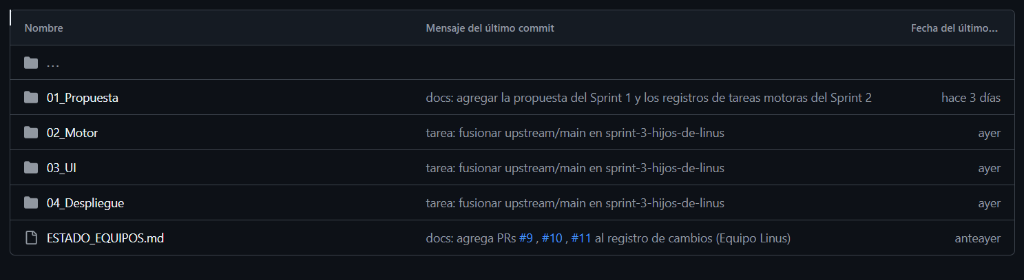
\includegraphics[width=0.85\textwidth]{informe_scratch_linus_p04_1024x280_bb5eb995.png}
\caption{Flujo Git del equipo Linus}
\label{fig:gal-lin-git}
\end{figure}

\begin{figure}[H]
\centering
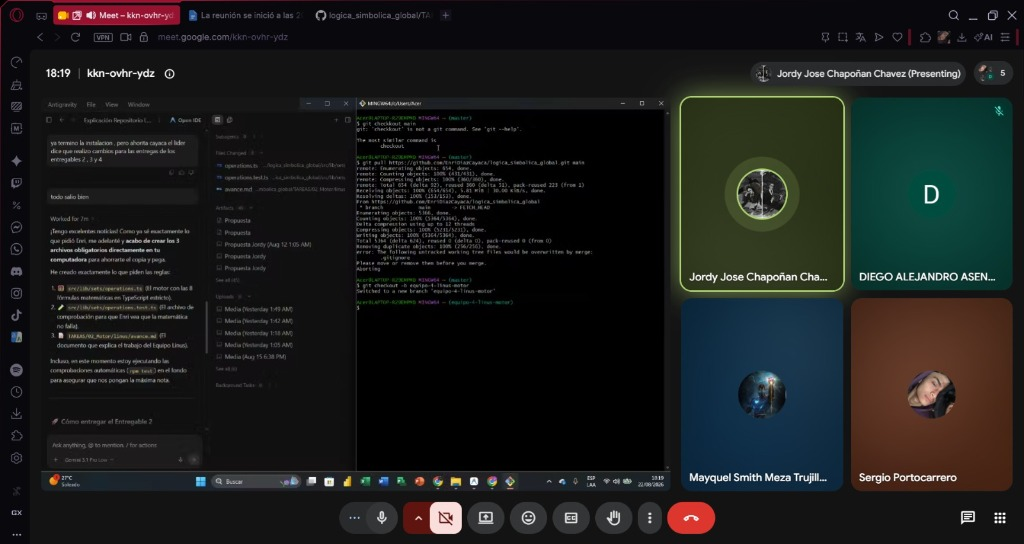
\includegraphics[width=0.9\textwidth]{informe_scratch_linus_p07_1024x544_a879fc66.jpeg}
\caption{Trabajo colaborativo del equipo Linus}
\label{fig:gal-lin-meet}
\end{figure}

\begin{figure}[H]
\centering
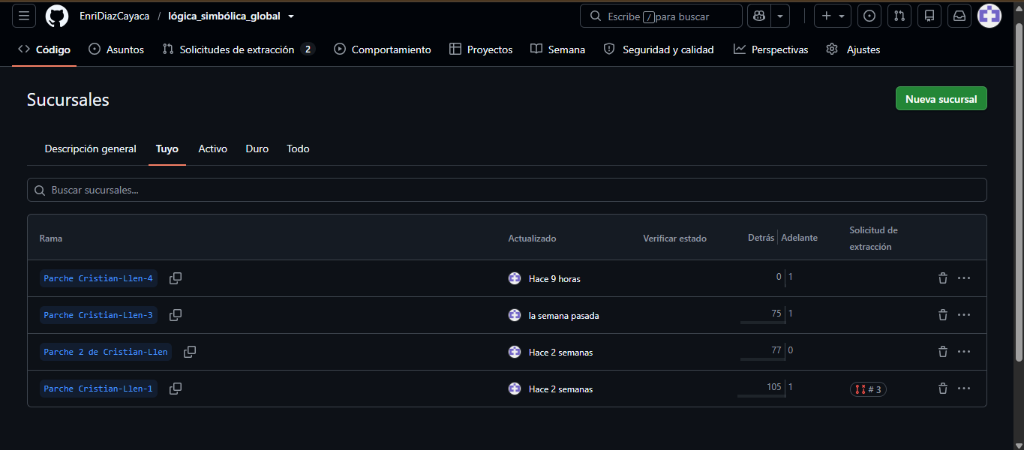
\includegraphics[width=0.9\textwidth]{informe_scratch_modusinnova_p08_1024x450_12adb3de.png}
\caption{Integraci\'on Vue del equipo Modus Innova}
\label{fig:gal-mod-vue}
\end{figure}

\begin{figure}[H]
\centering
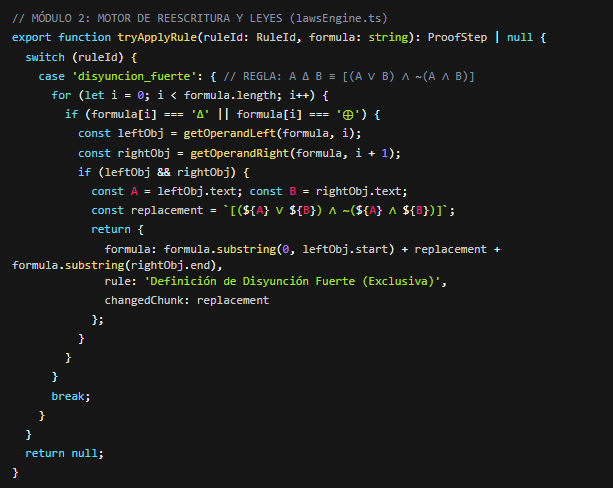
\includegraphics[width=0.9\textwidth]{informe_scratch_modusinnova_p14_613x488_6f3177e1.png}
\caption{Regla de disyunci\'on fuerte del equipo Modus Innova}
\label{fig:gal-mod-delta}
\end{figure}

\begin{figure}[H]
\centering
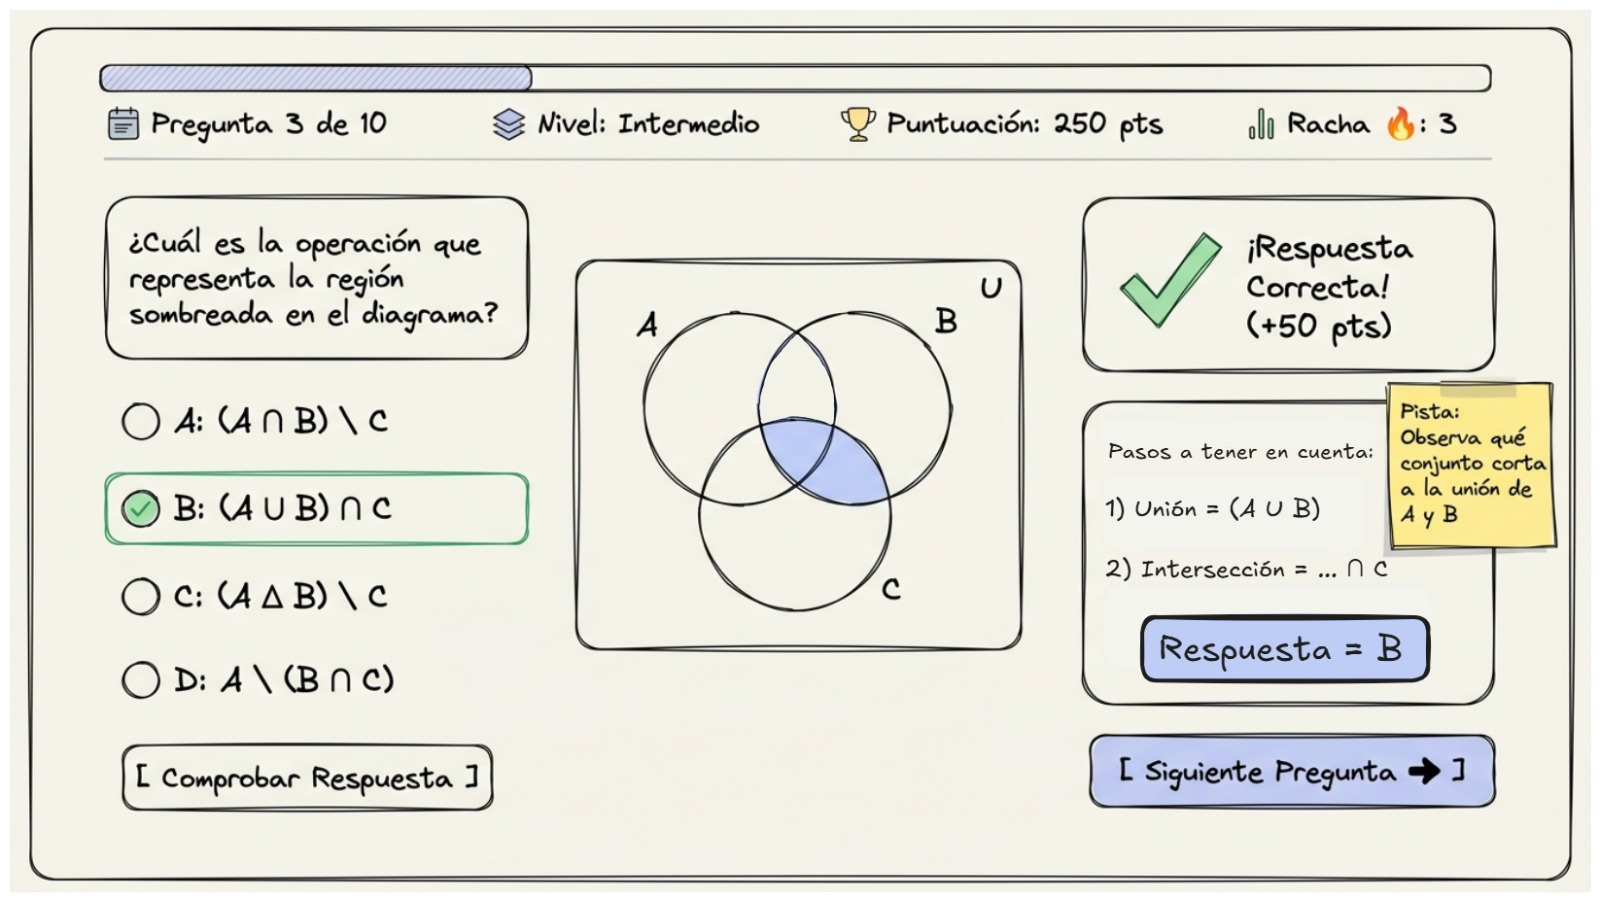
\includegraphics[width=0.48\textwidth]{propuesta_linus_propuesta-fernando.jpg}
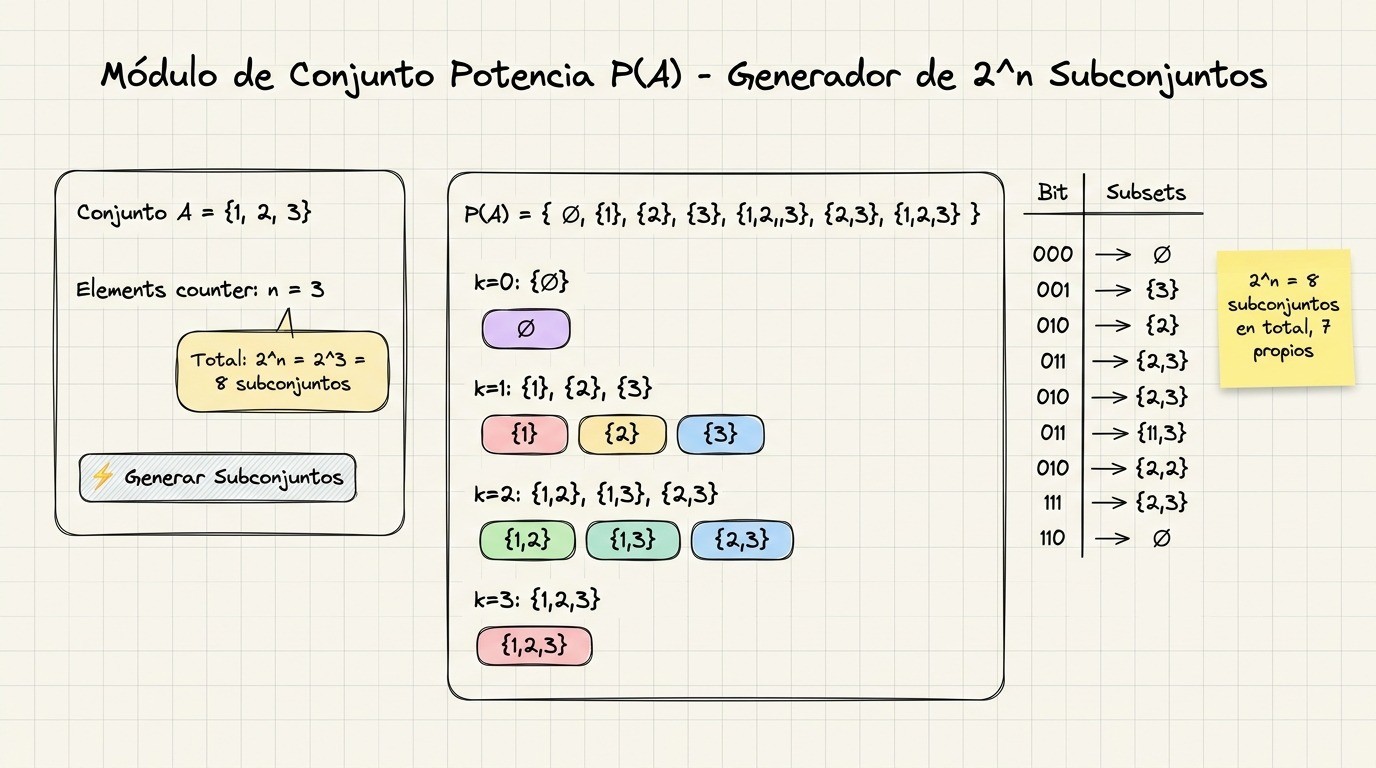
\includegraphics[width=0.48\textwidth]{propuesta_linus_propuesta-mike.jpg}
\caption{Bocetos Fernando y Mike (equipo Linus)}
\label{fig:gal-lin-boc2}
\end{figure}

\begin{figure}[H]
\centering
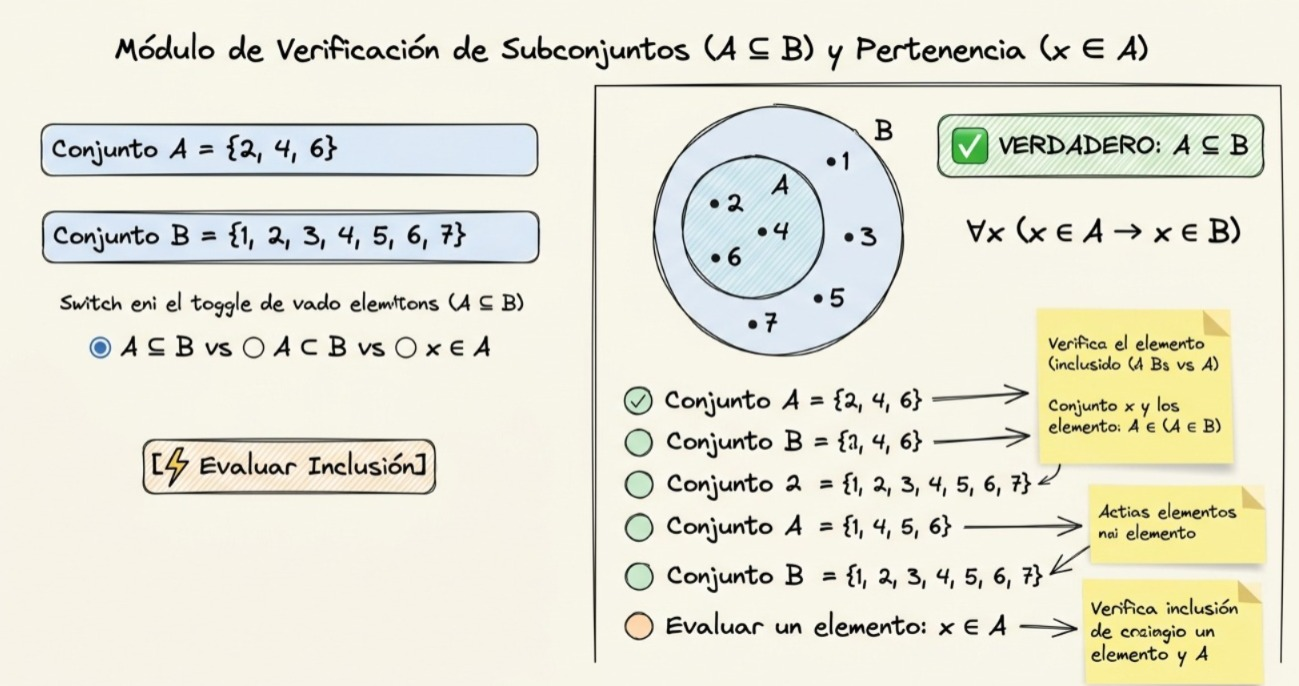
\includegraphics[width=0.48\textwidth]{propuesta_linus_propuesta-nio.jpg}
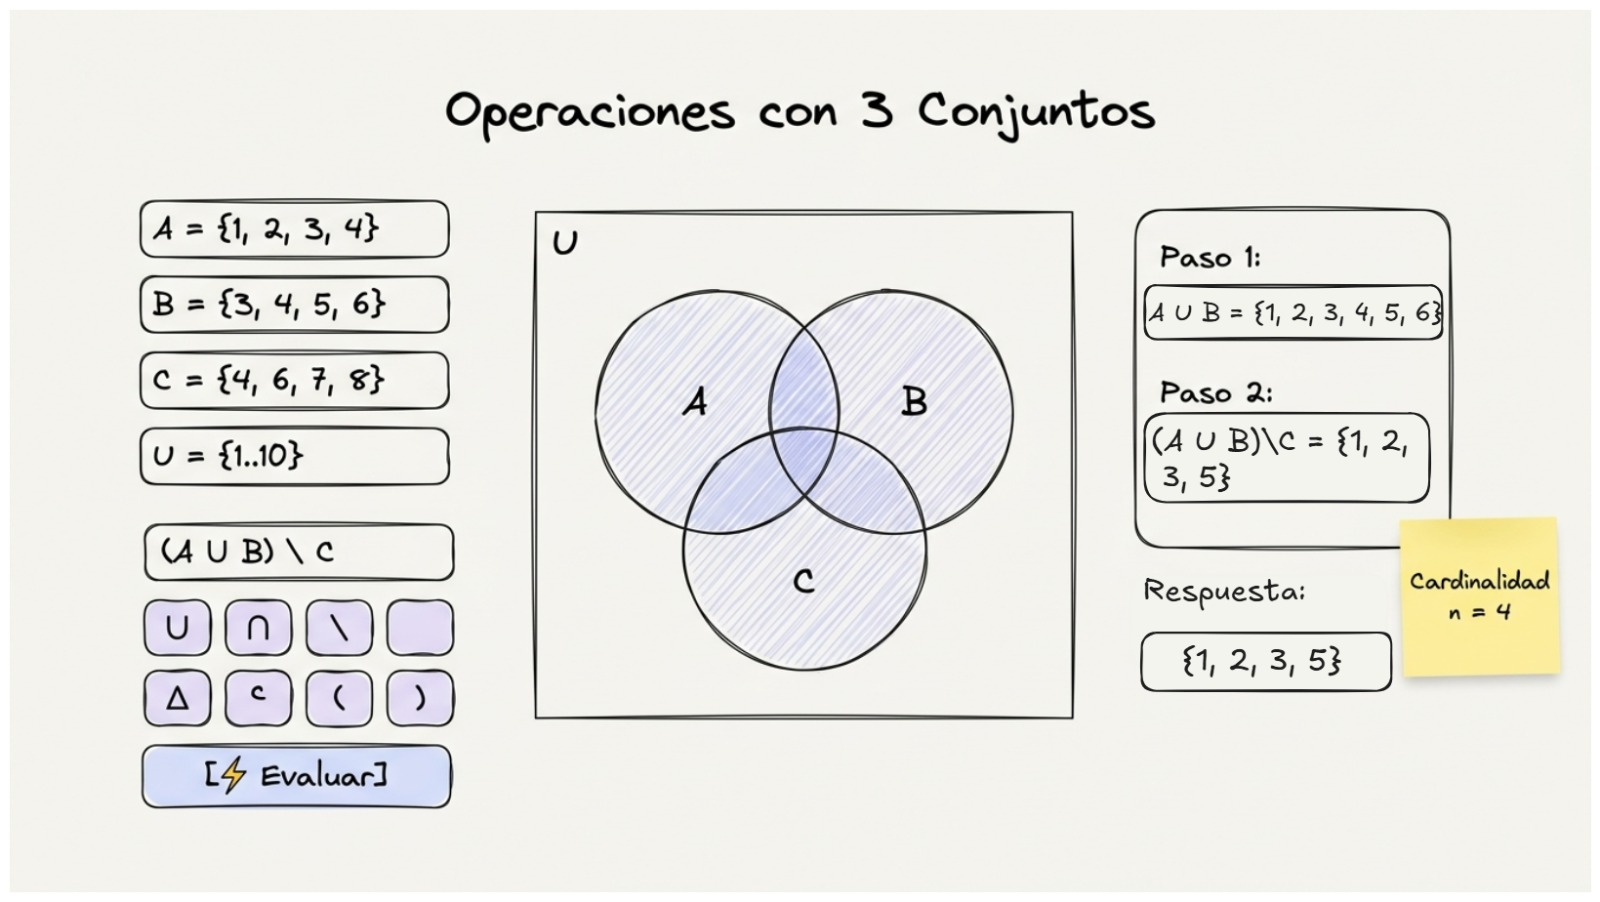
\includegraphics[width=0.48\textwidth]{propuesta_linus_propuesta-sergio.jpg}
\caption{Bocetos Nio y Sergio (equipo Linus)}
\label{fig:gal-lin-boc3}
\end{figure}

\begin{figure}[H]
\centering
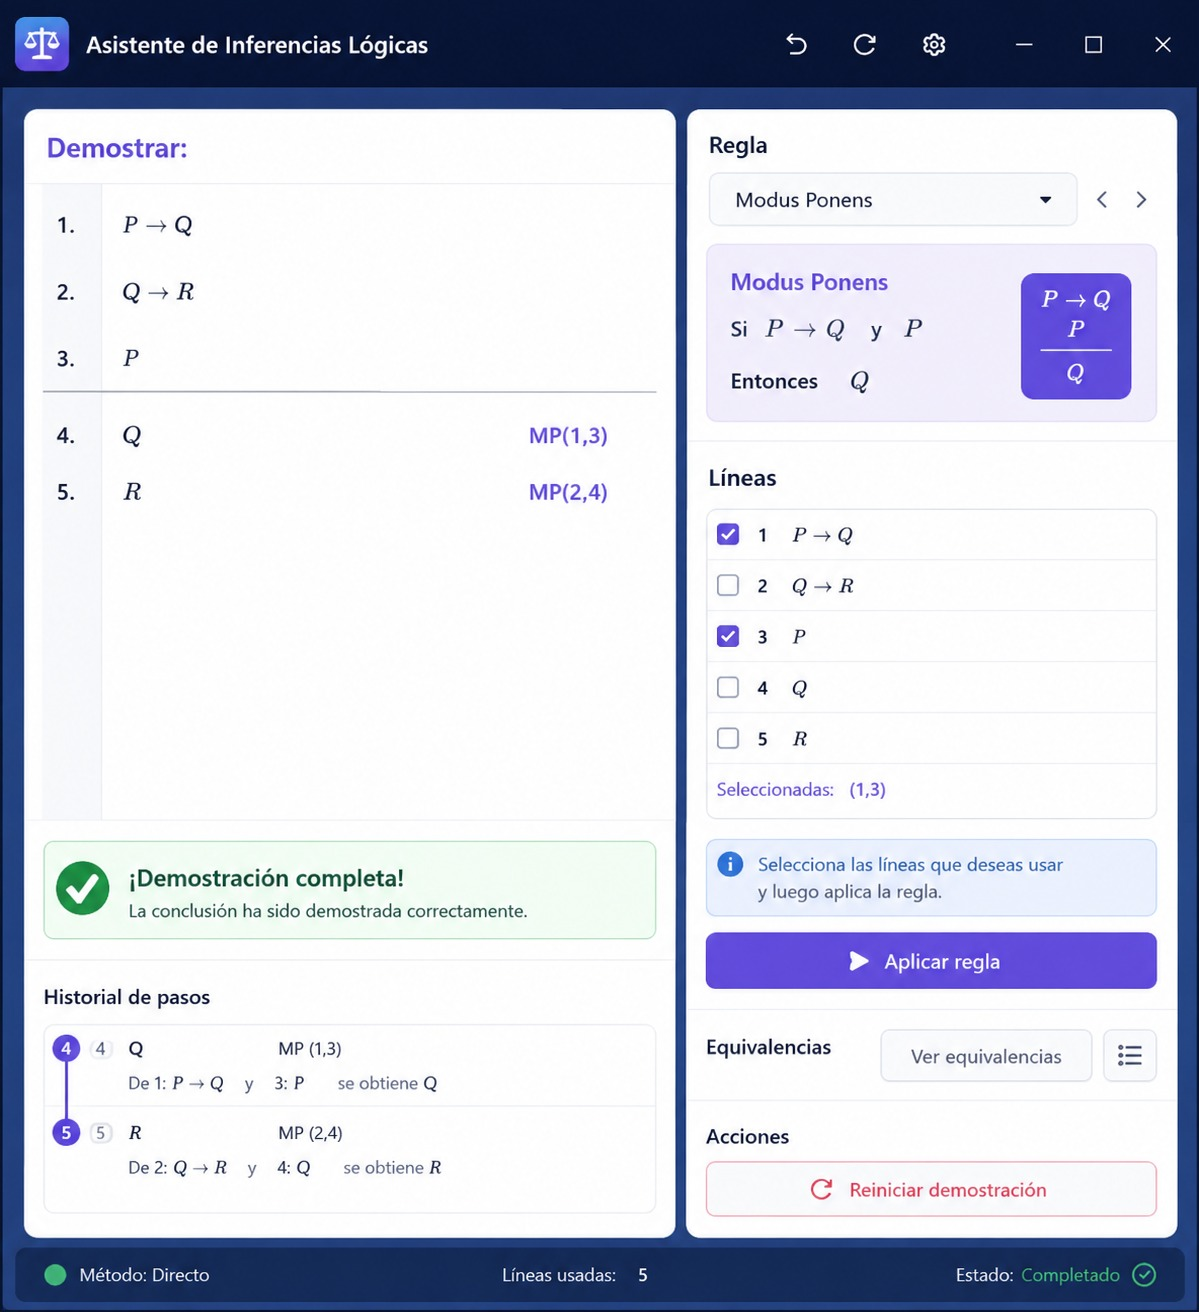
\includegraphics[width=0.85\textwidth]{propuesta_hijos_propuesta-morocho.jpeg}
\caption{Entorno de pr\'actica (equipo Hijos de Linus)}
\label{fig:gal-hijos-morocho}
\end{figure}

\begin{figure}[H]
\centering
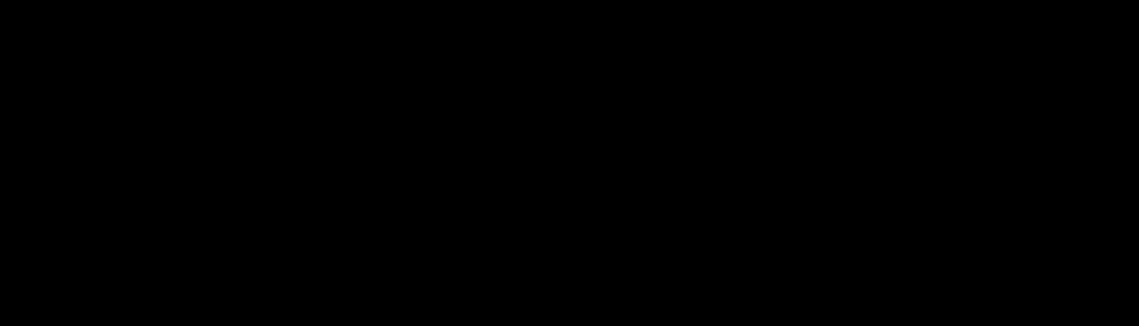
\includegraphics[width=0.9\textwidth]{informe_scratch_sinergia_p25_1139x326_547a68c9.png}
\caption{Cronograma Gantt del equipo Sinergia}
\label{fig:gal-gantt}
\end{figure}

\chapter{Cat\'alogo de ejercicios y progreso}
\label{ch:catalogo}
\section{Banco de 80 ejercicios}
El banco combina identificaci\'on de conectores, tablas de verdad, clasificaci\'on, leyes l\'ogicas y cuestionarios por bloques. Cada ejercicio indica dificultad (f\'acil, media, dif\'icil) y tema. La Tabla~\ref{tab:banco} resume la distribuci\'on.
\begin{table}[H]
\centering
\caption{Distribuci\'on del banco por tipo}
\label{tab:banco}
\begin{tabular}{lcc}
\toprule
Tipo & Cantidad & Ejemplo \\
\midrule
Identificaci\'on & 6 & $\lnot p$ es negaci\'on \\
Tablas de verdad & 10 & completar $p \lor q$ \\
Clasificaci\'on & 6 & $p \lor \lnot p$ es tautolog\'ia \\
Leyes l\'ogicas & 12 & $\lnot(p \land q)$ usa Morgan \\
Cuestionarios & 46 & bloques de 4 a 10 preguntas \\
\bottomrule
\end{tabular}
\end{table}
\section{Progreso}
El progreso persiste en el navegador con precisi\'on por tema, puntos, racha y logros. El panel de recomendaciones indica el tema con precisi\'on m\'as baja y enlaza a ejercicios filtrados de ese tema.
\chapter{Operaciones de conjuntos resueltas una por una}
\label{ch:conj-res}
Con $U = \{1,\ldots,10\}$, $A = \{1,2,3,4\}$, $B = \{3,4,5,6\}$ se obtiene $A \cup B = \{1,2,3,4,5,6\}$, $A \cap B = \{3,4\}$, $A \setminus B = \{1,2\}$, $B \setminus A = \{5,6\}$, $A^{c} = \{5,6,7,8,9,10\}$. Cada operaci\'on colorea su regi\'on en el diagrama: la uni\'on ilumina ambos c\'irculos, la intersecci\'on solo el lente central, la diferencia solo el lado correspondiente y el complemento todo el rect\'angulo $U$ salvo el c\'irculo. La potencia $P(\{1,2\}) = \{\emptyset, \{1\}, \{2\}, \{1,2\}\}$ tiene $2^{2} = 4$ elementos; en general $|P(A)| = 2^{|A|}$, por lo que con $|A| > 10$ la plataforma muestra la advertencia con el total en lugar de listar.

\chapter{Reglas de inferencia con ejemplo}
\label{ch:reglas-ej}
\begin{table}[H]
\centering
\caption{Once reglas con ejemplo corto}
\label{tab:reglas-ej}
\begin{tabular}{lll}
\toprule
Regla & Esquema & Ejemplo \\
\midrule
Modus Ponens & $p, p \to q \vdash q$ & Llueve, si llueve me mojo $\vdash$ me mojo \\
Modus Tollens & $\lnot q, p \to q \vdash \lnot p$ & No me mojo $\vdash$ no llueve \\
Silogismo hipot\'etico & $p \to q, q \to r \vdash p \to r$ & Transitividad \\
Silogismo disyuntivo & $p \lor q, \lnot p \vdash q$ & O pan o torta; no pan $\vdash$ torta \\
Adici\'on & $p \vdash p \lor q$ & Tengo pan $\vdash$ pan o torta \\
Simplificaci\'on & $p \land q \vdash p$ & Pan y torta $\vdash$ pan \\
Conjunci\'on & $p, q \vdash p \land q$ & Junci\'on de premisas \\
Dilema constructivo & $p \to q, r \to s, p \lor r \vdash q \lor s$ & Casos \\
Eliminaci\'on bicondicional & $p \leftrightarrow q \vdash p \to q$ & Descomposici\'on \\
Modus Ponens bicondicional & $p \leftrightarrow q, p \vdash q$ & Afirmaci\'on \\
Doble negaci\'on & $\lnot\lnot p \vdash p$ & Cancelaci\'on \\
\bottomrule
\end{tabular}
\end{table}
La falacia de afirmar el consecuente ($p \to q$, $q \vdash p$) es inv\'alida con contraejemplo $p = F$, $q = V$; la de negar el antecedente ($p \to q$, $\lnot p \vdash \lnot q$) tambi\'en es inv\'alida. El panel de trazabilidad las distingue de las v\'alidas mostrando la asignaci\'on que refuta.

\chapter{Cuantificadores evaluados elemento por elemento}
\label{ch:cuant-eval}
\begin{table}[H]
\centering
\caption{Evaluaci\'on de $\forall x \in \{1,2,3\}$ con $x$ par}
\begin{tabular}{cl|c}
\toprule
$x$ & $P(x)$ & Resultado \\
\midrule
1 & impar & $F$ \\
2 & par & $V$ \\
3 & impar & $F$ \\
\bottomrule
\end{tabular}
\end{table}
Como no todos los elementos satisfacen $P(x)$, la proposici\'on $\forall x\,P(x)$ es $F$ con contraejemplo $x = 1$, pues $P(1) = F$. En cambio $\exists x\,P(x)$ es $V$ con testigo $x = 2$. Para el rango $D = \{x \in \mathbb{Z} : 0 < x < 9\}$ con $x$ par, el primer contraejemplo vuelve a ser $x = 1$. La negaci\'on de De Morgan transforma $\lnot(\forall x\,P(x))$ en $\exists x\,\lnot P(x)$.

\chapter{Galer\'ia complementaria de evidencias}
\label{ch:galeria2}
\begin{figure}[H]
\centering

\includegraphics[width=0.9\textwidth]{informe_scratch_sinergia_p11_1142x370_e7fa07bc.png}
\caption{Parser recursivo del equipo Sinergia (detalle)}
\label{fig:gal2-parser}
\end{figure}

\begin{figure}[H]
\centering

\includegraphics[width=0.9\textwidth]{informe_scratch_sinergia_p13_1142x711_0aec1f8b.png}
\caption{Envoltura del \'arbol a Unicode (Sinergia)}
\label{fig:gal2-wrap}
\end{figure}

\begin{figure}[H]
\centering

\includegraphics[width=0.9\textwidth]{informe_scratch_sinergia_p15_1142x658_aed7f488.png}
\caption{Estado reactivo de la vista de tablas (Sinergia)}
\label{fig:gal2-estado}
\end{figure}

\begin{figure}[H]
\centering

\includegraphics[width=0.9\textwidth]{informe_scratch_sinergia_p17_1142x897_1d53bee2.png}
\caption{Propiedades computadas de la vista (Sinergia)}
\label{fig:gal2-computed}
\end{figure}

\begin{figure}[H]
\centering
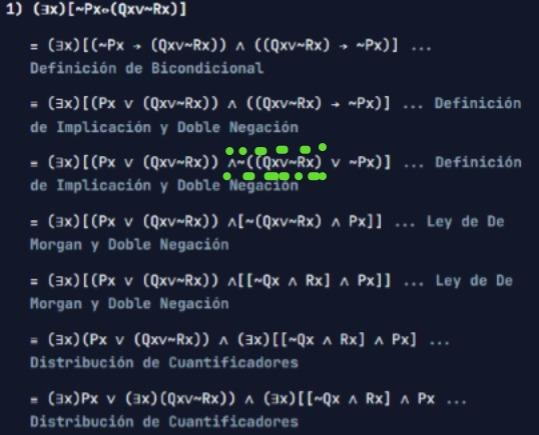
\includegraphics[width=0.9\textwidth]{informe_scratch_modusinnova_p09_539x435_0b0dfc19.jpeg}
\caption{Demostraci\'on paso a paso del motor de leyes (Modus Innova)}
\label{fig:gal2-leyes}
\end{figure}

\chapter{Verificaci\'on tabular de las leyes restantes}
\label{ch:leyes-tablas}
\begin{table}[H]
\centering
\caption{Idempotencia $p \land p \equiv p$}
\begin{tabular}{c|c}
\toprule
$p$ & $p \land p$ \\
\midrule
$V$ & $V$ \\
$F$ & $F$ \\
\bottomrule
\end{tabular}
\end{table}

\begin{table}[H]
\centering
\caption{Asociativa $(p \land q) \land r \equiv p \land (q \land r)$ (extracto, 8 filas en total)}
\begin{tabular}{ccc|c|c}
\toprule
$p$ & $q$ & $r$ & $(p \land q) \land r$ & $p \land (q \land r)$ \\
\midrule
$V$ & $V$ & $V$ & $V$ & $V$ \\
$V$ & $V$ & $F$ & $F$ & $F$ \\
$V$ & $F$ & $V$ & $F$ & $F$ \\
$F$ & $F$ & $F$ & $F$ & $F$ \\
\bottomrule
\end{tabular}
\end{table}

\begin{table}[H]
\centering
\caption{Distributiva $p \land (q \lor r)$ (8 filas, extracto)}
\begin{tabular}{ccc|c|c}
\toprule
$p$ & $q$ & $r$ & $p \land (q \lor r)$ & $(p \land q) \lor (p \land r)$ \\
\midrule
$V$ & $V$ & $V$ & $V$ & $V$ \\
$V$ & $V$ & $F$ & $V$ & $V$ \\
$V$ & $F$ & $F$ & $F$ & $F$ \\
$F$ & $V$ & $V$ & $F$ & $F$ \\
\bottomrule
\end{tabular}
\end{table}

\begin{table}[H]
\centering
\caption{Complemento: doble negaci\'on, contradicci\'on y tautolog\'ia}
\begin{tabular}{c|c|c|c}
\toprule
$p$ & $\lnot\lnot p$ & $p \land \lnot p$ & $p \lor \lnot p$ \\
\midrule
$V$ & $V$ & $F$ & $V$ \\
$F$ & $F$ & $F$ & $V$ \\
\bottomrule
\end{tabular}
\end{table}

\begin{table}[H]
\centering
\caption{Identidad con constantes $V$ y $F$}
\begin{tabular}{c|c|c|c|c}
\toprule
$p$ & $p \land V$ & $p \land F$ & $p \lor V$ & $p \lor F$ \\
\midrule
$V$ & $V$ & $F$ & $V$ & $V$ \\
$F$ & $F$ & $F$ & $V$ & $F$ \\
\bottomrule
\end{tabular}
\end{table}

\begin{table}[H]
\centering
\caption{Contraposici\'on $p \to q \equiv \lnot q \to \lnot p$}
\begin{tabular}{cc|c|c}
\toprule
$p$ & $q$ & $p \to q$ & $\lnot q \to \lnot p$ \\
\midrule
$V$ & $V$ & $V$ & $V$ \\
$V$ & $F$ & $F$ & $F$ \\
$F$ & $V$ & $V$ & $V$ \\
$F$ & $F$ & $V$ & $V$ \\
\bottomrule
\end{tabular}
\end{table}

\begin{table}[H]
\centering
\caption{Definici\'on $p \to q \equiv \lnot p \lor q$}
\begin{tabular}{cc|c|c}
\toprule
$p$ & $q$ & $p \to q$ & $\lnot p \lor q$ \\
\midrule
$V$ & $V$ & $V$ & $V$ \\
$V$ & $F$ & $F$ & $F$ \\
$F$ & $V$ & $V$ & $V$ \\
$F$ & $F$ & $V$ & $V$ \\
\bottomrule
\end{tabular}
\end{table}

\chapter{Recorrido visual completo del m\'odulo de tablas}
\label{ch:tablas-visual}
\begin{figure}[H]
\centering

\includegraphics[width=0.9\textwidth]{informe_scratch_sinergia_p02_1143x681_b6d55480.png}
\caption{Portada del informe original del equipo Sinergia}
\label{fig:v-sin-portada}
\end{figure}

\begin{figure}[H]
\centering

\includegraphics[width=0.9\textwidth]{informe_scratch_sinergia_p07_1142x314_1f242f3b.png}
\caption{Tipos del evaluador (material original Sinergia)}
\label{fig:v-sin-tipos}
\end{figure}

\begin{figure}[H]
\centering

\includegraphics[width=0.9\textwidth]{informe_scratch_sinergia_p08_1142x923_313c7ac1.png}
\caption{Tokenizador aut\'omata finito (Sinergia)}
\label{fig:v-sin-afd}
\end{figure}

\begin{figure}[H]
\centering

\includegraphics[width=0.9\textwidth]{informe_scratch_sinergia_p11_1142x473_443fddb8.png}
\caption{Parser recursivo, continuaci\'on (Sinergia)}
\label{fig:v-sin-parser2}
\end{figure}

\begin{figure}[H]
\centering

\includegraphics[width=0.9\textwidth]{informe_scratch_sinergia_p15_1142x607_cfbbede0.png}
\caption{Estado reactivo de la vista (Sinergia)}
\label{fig:v-sin-react}
\end{figure}

\begin{figure}[H]
\centering

\includegraphics[width=0.9\textwidth]{informe_scratch_sinergia_p19_1142x101_d92c97bf.png}
\caption{Acceso al manual de usuario (Sinergia)}
\label{fig:v-sin-acceso}
\end{figure}

\begin{figure}[H]
\centering
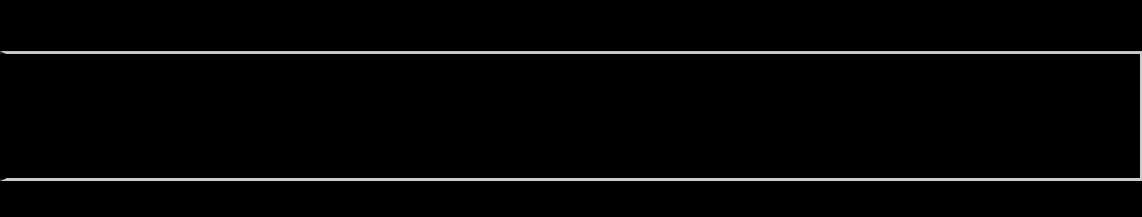
\includegraphics[width=0.9\textwidth]{informe_scratch_sinergia_p27_1142x217_5fe82248.png}
\caption{Pruebas del evaluador (Sinergia)}
\label{fig:v-sin-tests}
\end{figure}

\chapter{Conjuntos: las siete operaciones con resultados}
\label{ch:conj-siete}
Con $U = \{1,\ldots,10\}$, $A = \{1,2,3,4\}$, $B = \{3,4,5,6\}$:
\begin{table}[H]
\centering
\caption{Resultados de las siete operaciones}
\begin{tabular}{ll}
\toprule
Operaci\'on & Resultado \\
\midrule
$A \cup B$ & $\{1,2,3,4,5,6\}$ \\
$A \cap B$ & $\{3,4\}$ \\
$A \setminus B$ & $\{1,2\}$ \\
$B \setminus A$ & $\{5,6\}$ \\
$A^{c}$ & $\{5,6,7,8,9,10\}$ \\
$B^{c}$ & $\{1,2,7,8,9,10\}$ \\
$P(\{1,2\})$ & $\{\emptyset,\{1\},\{2\},\{1,2\}\}$ \\
\bottomrule
\end{tabular}
\end{table}

\begin{table}[H]
\centering
\caption{Potencia $P(\{1,2,3\})$ con $2^{3} = 8$ elementos}
\begin{tabular}{c}
\toprule
Subconjuntos \\
\midrule
$\emptyset$ \\
$\{1\}, \{2\}, \{3\}$ \\
$\{1,2\}, \{1,3\}, \{2,3\}$ \\
$\{1,2,3\}$ \\
\bottomrule
\end{tabular}
\end{table}

\chapter{Trazabilidad completa de un Modus Ponens}
\label{ch:mp-full}
Para $P \to Q$, $P \vdash Q$ el motor produce: L\'inea 1: $P \to Q$ (premisa), L\'inea 2: $P$ (premisa), L\'inea 3: $Q$ (Modus Ponens de 1 y 2). El \'arbol de $P \to Q$ tiene ra\'iz $\to$ con hijos $P$ y $Q$. La traducci\'on a lenguaje natural con mapa $P \mapsto$ ``Llueve'' y $Q \mapsto$ ``Me mojo'' produce \textit{Si llueve, entonces me mojo; llueve; por tanto, me mojo}. El historial guarda el ejercicio y permite restaurarlo en un clic.

\chapter{Disyunci\'on fuerte y De Morgan cuantificacional}
\label{ch:delta}
La disyunci\'on fuerte se define $p \,\Delta\, q \equiv (p \lor q) \land \lnot(p \land q)$: es $V$ cuando exactamente una es $V$.
\begin{table}[H]
\centering
\caption{Tabla de $p \,\Delta\, q$}
\begin{tabular}{cc|c}
\toprule
$p$ & $q$ & $p \,\Delta\, q$ \\
\midrule
$V$ & $V$ & $F$ \\
$V$ & $F$ & $V$ \\
$F$ & $V$ & $V$ \\
$F$ & $F$ & $F$ \\
\bottomrule
\end{tabular}
\end{table}
De Morgan cuantificacional: $\lnot(\forall x\,P(x)) \equiv \exists x\,\lnot P(x)$. Con $D = \{1,2,3\}$ y $P(x)$ par, $\forall x\,P(x)$ es $F$ y su negaci\'on equivale a $\exists x\,\lnot P(x)$, testigo $x = 1$.

\begin{figure}[H]
\centering
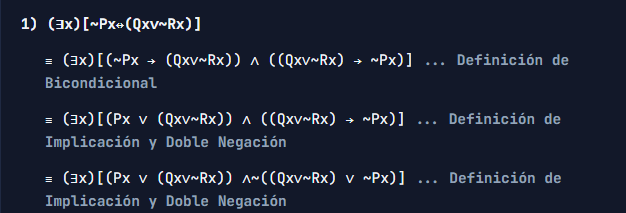
\includegraphics[width=0.9\textwidth]{informe_scratch_modusinnova_p09_626x213_e54a46e2.png}
\caption{Demostraci\'on de leyes, segunda parte (Modus Innova)}
\label{fig:v-mod-leyes2}
\end{figure}

\chapter{Veinte ejercicios representativos con soluci\'on}
\label{ch:ej20}
\begin{enumerate}[leftmargin=*]
\item Identificar $\lnot p$: respuesta \textit{Negaci\'on}, pues $\lnot$ invierte el valor.
\item Identificar $p \land q$: \textit{Conjunci\'on}, $V$ solo si ambas son $V$.
\item Identificar $p \lor q$: \textit{Disyunci\'on}, $F$ solo si ambas son $F$.
\item Identificar $p \to q$: \textit{Condicional}, $F$ solo con $V \to F$.
\item Identificar $p \leftrightarrow q$: \textit{Bicondicional}, $V$ si coinciden.
\item Clasificar $p \lor \lnot p$: \textit{tautolog\'ia}.
\item Clasificar $p \land \lnot p$: \textit{contradicci\'on}.
\item Clasificar $p \to q$: \textit{contingencia}.
\item Ley de $\lnot(p \land q)$: \textit{Morgan}.
\item Ley de $p \land (p \lor q)$: \textit{Absorci\'on}.
\item Tabla de $p \lor q$: 4 filas.
\item Tabla de $p \land q \to r$: 8 filas.
\item Cuantificador $\forall$ en $\{2,4,6\}$ par: $V$.
\item Cuantificador $\exists$ en $\{1,3,5\}$ par: $F$.
\item Conjunto $A \cup B$ con ejemplo: $\{1,\ldots,6\}$.
\item Conjunto $A \cap B$: $\{3,4\}$.
\item Inferencia $P \to Q, P$: $Q$ por Modus Ponens.
\item Tautolog\'ia $(p \land q) \to p$: siempre $V$.
\item Contingencia $p \lor q$: mixta.
\item De Morgan cuantificacional: $\lnot\forall \equiv \exists\lnot$.
\end{enumerate}

\chapter{Precedencia y notaciones aceptadas}
\label{ch:precedencia}
La precedencia del motor es $\lnot > \land > \lor > \to > \leftrightarrow$. As\'i, $P \land Q \to R$ se lee $(P \land Q) \to R$ y no $P \land (Q \to R)$; $\lnot P \lor Q$ se lee $(\lnot P) \lor Q$.
\begin{table}[H]
\centering
\caption{Notaciones aceptadas por el motor}
\label{tab:notaciones}
\begin{tabular}{lll}
\toprule
Conectivo & S\'imbolo & ASCII y palabras \\
\midrule
Negaci\'on & $\lnot$ & \texttt{!, NOT, no} \\
Conjunci\'on & $\land$ & \texttt{\&\&, AND} \\
Disyunci\'on & $\lor$ & \texttt{||, OR} \\
Condicional & $\to$ & \texttt{->, IMPL} \\
Bicondicional & $\leftrightarrow$ & \texttt{<->, BICOND} \\
\bottomrule
\end{tabular}
\end{table}

\chapter{Traducci\'on a lenguaje natural con ejemplos}
\label{ch:traductor}
\begin{table}[H]
\centering
\caption{Cinco traducciones con mapa}
\label{tab:trad}
\begin{tabular}{ll}
\toprule
F\'ormula & Traducci\'on con $P \mapsto$ Llueve, $Q \mapsto$ Me mojo \\
\midrule
$P \to Q$ & Si llueve, entonces me mojo \\
$P \land Q$ & Llueve y me mojo \\
$P \lor Q$ & Llueve o me mojo \\
$\lnot P$ & No es cierto que llueve \\
$P \leftrightarrow Q$ & Llueve si y solo si me mojo \\
\bottomrule
\end{tabular}
\end{table}
La exportaci\'on acad\'emica genera el paso a paso en \LaTeX\ y Markdown con un clic, lista para incluir en trabajos con entorno \texttt{aligned} y citas.

\chapter{Dominios y predicados del m\'odulo de cuantificadores}
\label{ch:dominios}
\begin{table}[H]
\centering
\caption{Formatos de dominio $D \subset \mathbb{Z}$}
\label{tab:dominios}
\begin{tabular}{ll}
\toprule
Formato & Ejemplo \\
\midrule
Lista & \texttt{1, 2, 3, 4, 5} \\
Rango & \texttt{0 < x < 9} equivale a $D = \{x \in \mathbb{Z} : 0 < x < 9\}$ \\
Mixto & combinaci\'on validada por el motor estricto \\
\bottomrule
\end{tabular}
\end{table}
\begin{table}[H]
\centering
\caption{Predicados predefinidos}
\label{tab:predicados}
\begin{tabular}{ll}
\toprule
Predicado & Lectura \\
\midrule
$x$ es par & $x \% 2 === 0$ \\
$x$ es impar & $x \% 2 !== 0$ \\
$x$ es primo & divisores solo $1$ y $x$ \\
$x$ mayor que 2 & $x > 2$ \\
$x$ positivo & $x > 0$ \\
\bottomrule
\end{tabular}
\end{table}

\chapter{Preguntas frecuentes extendidas}
\label{ch:faq2}
\begin{description}[leftmargin=*]
\item[Por qu\'e mi tabla tiene 8 filas?] Porque hay 3 variables: $2^{3} = 8$ combinaciones.
\item[Por qu\'e la implicaci\'on me da $V$ con antecedente $F$?] Por definici\'on material: $F \to Q$ siempre es $V$.
\item[Qu\'e significa \textit{V\'alida (Ind.)}?] V\'alida por m\'etodo indirecto cuando la directa no aplica.
\item[D\'onde veo mi precisi\'on?] En \textit{Progreso}, por tema, con recomendaci\'on.
\item[Puedo desactivar variables?] S\'i, con el interruptor de cada variable.
\item[Qu\'e es $D \subset \mathbb{Z}$?] Dominio finito de enteros donde se eval\'ua.
\item[Qu\'e es un testigo?] Elemento que hace $V$ a un $\exists$.
\item[Qu\'e es un contraejemplo?] Asignaci\'on que refuta validez.
\item[C\'omo cito la plataforma?] Ver bibliograf\'ia: Vue, Vite y l\'ogica (Copi, Hurley).
\item[Funciona sin internet?] La versi\'on publicada requiere conexi\'on; la local no tras instalar.
\end{description}

\chapter{Objetivos de aprendizaje y mapa del s\'ilabo}
\label{ch:silabo}
\begin{table}[H]
\centering
\caption{Cobertura del s\'ilabo MATG1001}
\label{tab:silabo}
\begin{tabular}{lll}
\toprule
Resultado & Contenido & M\'odulo \\
\midrule
D1 & Proposicional y tablas & Tablas, Aprender \\
D2 & Inferencia & Inferencias, Leyes \\
D3 & Conjuntos y predicados & Conjuntos, Cuantificadores \\
\bottomrule
\end{tabular}
\end{table}
Cada resultado se practica con motores verificables y 80 ejercicios con retroalimentaci\'on inmediata.

\chapter{Recorrido guiado completo: un conector y una ley}
\label{ch:walkthrough}
\section{Conector: $p \land q$ en cuatro pasos}
\textit{Definici\'on:} la conjunci\'on solo es $V$ si ambas son $V$. \textit{Ejemplo:} con $p = V$, $q = F$ el resultado es $F$. \textit{Ejercicio:} identificar $p \land q$ entre cinco opciones. \textit{Soluci\'on:} es conjunci\'on porque el operador principal es $\land$, aunque un miembro est\'e negado seguir\'ia siendo conjunci\'on si el operador principal no cambia.
\section{Ley: Morgan en cuatro pasos}
\textit{Definici\'on:} $\lnot(p \land q) \equiv \lnot p \lor \lnot q$. \textit{Ejemplo:} con $p = V$, $q = F$ ambos lados dan $V$. \textit{Ejercicio:} decidir si la equivalencia es correcta. \textit{Soluci\'on:} ambos lados coinciden porque al negar se intercambia $\land$ por $\lor$.

\chapter{Diez ejercicios resueltos paso a paso}
\label{ch:diez}
\begin{enumerate}[leftmargin=*]
\item $\lnot p$ es \textit{negaci\'on}: $\lnot$ invierte el valor de verdad.
\item $p \land q$ es \textit{conjunci\'on}: $V$ solo si ambas son $V$.
\item $p \lor q$ es \textit{disyunci\'on}: $F$ solo si ambas son $F$.
\item $p \to q$ es \textit{condicional}: $F$ solo con $V \to F$.
\item $p \leftrightarrow q$ es \textit{bicondicional}: $V$ si coinciden.
\item $\lnot p \lor q$ tiene operador principal $\lor$: es \textit{disyunci\'on} aunque un miembro est\'e negado.
\item $p \lor \lnot p$ se clasifica \textit{tautolog\'ia} por tabla de 2 filas.
\item $p \land \lnot p$ se clasifica \textit{contradicci\'on}.
\item $\lnot(p \land q)$ usa la \textit{ley de Morgan}.
\item $p \land (p \lor q)$ usa la \textit{ley de absorci\'on} y se reduce a $p$.
\end{enumerate}

\chapter{Nodos del \'arbol sint\'actico y lectura del Venn}
\label{ch:ast-venn}
\begin{table}[H]
\centering
\caption{Nodos del AST}
\begin{tabular}{ll}
\toprule
Nodo & Lectura \\
\midrule
variable & $p$, $q$, $r$ \\
NO & $\lnot p$ \\
Y & $p \land q$ \\
O & $p \lor q$ \\
ENTONCES & $p \to q$ \\
SI\_Y\_SOLO\_SI & $p \leftrightarrow q$ \\
\bottomrule
\end{tabular}
\end{table}
Para leer el Venn: el rect\'angulo es $U$; el c\'irculo izquierdo es $A$; el derecho es $B$; el lente central es $A \cap B$; lo exterior a ambos c\'irculos pero interior al rect\'angulo es $U \setminus (A \cup B)$.

\chapter{Paneles de progreso y lista de verificaci\'on docente}
\label{ch:prog-check}
El progreso muestra precisi\'on por tema, puntos, racha y logros con recomendaci\'on del tema m\'as d\'ebil y enlace a ejercicios filtrados. Lista de verificaci\'on docente: instalar dependencias, verificar \textit{Crear tabla de verdad}, probar Modus Ponens, evaluar un $\forall$ con rango, calcular una potencia y exportar una demostraci\'on a \LaTeX.


\chapter{Anatom\'ia de cada pantalla (glosario visual)}
\label{ch:anatomia}
\section{Tablas: cada elemento}
La pantalla de Tablas contiene: cabecera con t\'itulo y subt\'itulo; tarjeta de entrada con etiqueta, campo monoespaciado y bot\'on \textbf{Crear tabla de verdad}; tarjeta \textit{Variables proposicionales} con un interruptor por variable; tarjeta \textit{Conectores l\'ogicos} con cinco botones con s\'imbolo y etiqueta; tarjeta de clasificaci\'on con color verde, rojo o \'ambar; tabla de verdad con columnas de variables, subexpresiones y Resultado; y tarjeta de explicaci\'on con lista numerada y bot\'on \textit{Ver resoluci\'on paso a paso}. La Figura~\ref{fig:anat-sin-estado} muestra el estado reactivo original.
\begin{figure}[H]
\centering

\includegraphics[width=0.9\textwidth]{informe_scratch_sinergia_p15_1142x607_cfbbede0.png}
\caption{Estado reactivo de la vista de tablas (material original Sinergia)}
\label{fig:anat-sin-estado}
\end{figure}
\section{Conjuntos: cada elemento}
La pantalla de Conjuntos contiene: navegaci\'on con volver e insignia del equipo; cabecera con t\'itulo y subt\'itulo; tarjeta \textit{Define tus conjuntos} con tres campos ($U$, $A$, $B$); tarjeta de operaciones con siete botones y sub-selector de potencia; diagrama de Venn; tarjeta de resultado con notaci\'on de conjuntos y total $2^{n}$; tarjeta de propiedades con insignias; y verificador de pertenencia con $\in$/$\notin$.
\section{Inferencias: cada elemento}
La pantalla de Inferencias contiene: cabecera con t\'itulo \textit{Explorador de Inferencias L\'ogicas} e insignia del equipo; bot\'on de historial; tres pesta\~nas (Simbolog\'ia Formal, Lenguaje Natural, \'Arbol Sint\'actico); formulario con premisas numeradas y conclusi\'on; indicador de resultado; panel de trazabilidad con l\'ineas base y regla; y traductor con mapa de variables.
\section{Cuantificadores: cada elemento}
La pantalla de Cuantificadores contiene: cabecera con icono $\forall\exists$; dos pesta\~nas (Cuantificadores, Distribuci\'on y Leyes); selector Para todo/Existe; dominio $D \subset \mathbb{Z}$ con ayuda de lista y rango; predicado $p(x)$ con interruptor Libre; s\'imbolos r\'apidos; botones Evaluar y ejemplos; resultado con contraejemplo o testigo; trazabilidad por elemento; De Morgan; y resolutor paso a paso con cat\'alogo de 12 leyes.
\begin{figure}[H]
\centering

\includegraphics[width=0.9\textwidth]{informe_scratch_sinergia_p12_1142x632_cf6d23c8.png}
\caption{Evaluaci\'on sem\'antica, continuaci\'on (material original Sinergia)}
\label{fig:anat-sin-eval2}
\end{figure}
\begin{figure}[H]
\centering

\includegraphics[width=0.9\textwidth]{informe_scratch_sinergia_p17_1142x458_12b2a8af.png}
\caption{Propiedades computadas, continuaci\'on (material original Sinergia)}
\label{fig:anat-sin-comp2}
\end{figure}

\chapter{Operaci\'on y mantenimiento para el docente}
\label{ch:mantenimiento}
Para publicar cambios de contenido, edite \texttt{src/content/site.json} por m\'odulo (cada uno con su interruptor \texttt{modoLiteral} que elige s\'imbolos o palabras) y regenere la plantilla de edici\'on. Valide con la suite de 189 pruebas antes de publicar. La Figura~\ref{fig:logo} muestra el logo institucional disponible para portadas alternativas.
\begin{figure}[H]
\centering

\includegraphics[width=0.35\textwidth]{public_logo.jpg}
\caption{Logo institucional LogiLearn}
\label{fig:logo}
\end{figure}


\chapter{Errores frecuentes por ley y soluciones razonadas}
\label{ch:errores-ley}
\begin{description}[leftmargin=*]
\item[Idempotencia.] Error: creer que $p \land p$ es m\'as fuerte que $p$. Soluci\'on: la tabla muestra identidad total.
\item[Asociativa.] Error: pensar que $(p \land q) \lor r$ equivale a $p \land (q \lor r)$. Soluci\'on: solo vale con el mismo operador.
\item[Conmutativa.] Error: aplicarla a $\to$. Soluci\'on: $p \to q$ no equivale a $q \to p$; use contraposici\'on.
\item[Distributiva.] Error: distribuir $\to$ como si fuera $\land$. Soluci\'on: conserve solo las dos formas v\'alidas y lea la nota.
\item[Absorci\'on.] Error: no reconocer el patr\'on con t\'erminos extra. Soluci\'on: identifique $p$ repetida.
\item[Morgan.] Error: negar sin intercambiar el operador. Soluci\'on: $\land$ pasa a $\lor$ siempre.
\item[Identidad.] Error: confundir neutro con absorbente. Soluci\'on: $V$ es neutro de $\land$ pero absorbente de $\lor$.
\item[Contraposici\'on.] Error: invertir sin negar. Soluci\'on: niegue ambos lados adem\'as de invertir.
\item[Exportaci\'on.] Error: aplanar $(p \land q) \to r$ como $p \land (q \to r)$. Soluci\'on: anide $p \to (q \to r)$.
\item[Definici\'on.] Error: definir $\leftrightarrow$ con un solo condicional. Soluci\'on: requiere la conjunci\'on de ambos sentidos.
\end{description}

\chapter{Soluciones razonadas de los diez ejercicios}
\label{ch:sol10}
\begin{enumerate}[leftmargin=*]
\item $\lnot p$: el s\'imbolo $\lnot$ antepuesto invierte el valor; con $p = V$ da $F$.
\item $p \land q$: con $p = V$, $q = F$ da $F$ porque basta un $F$.
\item $p \lor q$: con $p = V$, $q = F$ da $V$ porque basta un $V$.
\item $p \to q$: con $p = V$, $q = F$ da $F$, \'unico caso falso.
\item $p \leftrightarrow q$: con valores iguales da $V$, distintos da $F$.
\item $\lnot p \lor q$: el operador principal es $\lor$, luego es disyunci\'on.
\item $p \lor \lnot p$: tabla de 2 filas todo $V$, tautolog\'ia.
\item $p \land \lnot p$: tabla todo $F$, contradicci\'on.
\item $\lnot(p \land q)$: Morgan da $\lnot p \lor \lnot q$.
\item $p \land (p \lor q)$: absorci\'on da $p$.
\end{enumerate}

\chapter{Ampliaci\'on del traductor y del dominio}
\label{ch:trad-dom}
\begin{table}[H]
\centering
\caption{Otras cinco traducciones}
\begin{tabular}{ll}
\toprule
F\'ormula & Traducci\'on \\
\midrule
$P \land (Q \lor R)$ & Llueve y (me mojo o truena) \\
$\forall x\,P(x)$ & Para todo $x$, $x$ es par \\
$\exists x\,P(x)$ & Existe $x$ tal que $x$ es par \\
$\lnot\forall x\,P(x)$ & No todos son pares (equivale a $\exists x\,\lnot P(x)$) \\
$A \cup B$ & Elementos que est\'an en $A$ o en $B$ \\
\bottomrule
\end{tabular}
\end{table}
Flujo completo de rango: escriba \texttt{0 < x < 9}, active \textit{Libre} con $x \% 2 === 0$, pulse \textbf{Evaluar}: el motor expande $D = \{1,\ldots,8\}$, eval\'ua cada elemento y reporta $F$ con contraejemplo $x = 1$.

\chapter{Cat\'alogo completo del banco de ejercicios}
\label{ch:banco80}
El banco contiene 45 ejercicios tipados con fuente bibliogr\'afica (Copi, Hurley y elaboraci\'on propia). Cada fila indica identificador, categor\'ia, nivel, proposici\'on y respuesta correcta. Las explicaciones paso a paso aparecen en la plataforma al pulsar \textit{Soluci\'on}.
\begin{center}
\begin{longtable}{lllll}
\caption{Cat\'alogo del banco (45 ejercicios registrados)} \\
\toprule
ID & Categor\'ia & Nivel & Proposici\'on & Respuesta \\
\midrule
\endfirsthead
\caption{Cat\'alogo del banco (continuaci\'on)} \\
\toprule
ID & Categor\'ia & Nivel & Proposici\'on & Respuesta \\
\midrule
\endhead

id-1 & IDENTIFICACIÓN & facil & $ \textbackslash\{\}lnot $(p $ \textbackslash\{\}land $ (q $ \textbackslash\{\}lor $ $ \textbackslash\{\}lnot $r)) & Negación \\
id-2 & IDENTIFICACIÓN & medio & ((p $ \textbackslash\{\}to $ q) $ \textbackslash\{\}land $ (q $ \textbackslash\{\}to $ r)) $ \textbackslash\{\}land $ $ \textbackslash\{\}lnot $(p $ \textbackslash\{\}to $ r) & Conjunción \\
id-3 & IDENTIFICACIÓN & medio & ((p $ \textbackslash\{\}land $ q) $ \textbackslash\{\}to $ r) $ \textbackslash\{\}to $ ((p $ \textbackslash\{\}to $ r) $ \textbackslash\{\}lor $ (q $ \textbackslash\{\}to $ r)) & Condicional \\
id-4 & IDENTIFICACIÓN & dificil & ((p $ \textbackslash\{\}lor $ $ \textbackslash\{\}lnot $q) $ \textbackslash\{\}leftrightarrow $ ($ \textbackslash\{\}lnot $p $ \textbackslash\{\}land $ r)) $ \textbackslash\{\}leftrightarrow $ (q $ \textbackslash\{\}to $ (r $ \textbackslash\{\}lor $ s)) & Bicondicional \\
id-5 & IDENTIFICACIÓN & dificil & $ \textbackslash\{\}lnot $(((p $ \textbackslash\{\}to $ q) $ \textbackslash\{\}land $ (r $ \textbackslash\{\}to $ s)) $ \textbackslash\{\}to $ ((p $ \textbackslash\{\}lor $ r) $ \textbackslash\{\}to $ (q $ \textbackslash\{\}lor $ s))) & Negación \\
id-6 & IDENTIFICACIÓN & medio & (((p $ \textbackslash\{\}lor $ q) $ \textbackslash\{\}land $ $ \textbackslash\{\}lnot $p) $ \textbackslash\{\}to $ q) $ \textbackslash\{\}lor $ ((p $ \textbackslash\{\}land $ q) $ \textbackslash\{\}leftrightarrow $ (q $ \textbackslash\{\}land $ p)) & Disyunción \\
id-7 & IDENTIFICACIÓN & dificil & ((p $ \textbackslash\{\}to $ (q $ \textbackslash\{\}to $ r)) $ \textbackslash\{\}land $ (p $ \textbackslash\{\}to $ q)) $ \textbackslash\{\}to $ (p $ \textbackslash\{\}to $ r) & Condicional \\
id-8 & IDENTIFICACIÓN & medio & $ \textbackslash\{\}lnot $p $ \textbackslash\{\}land $ ((q $ \textbackslash\{\}leftrightarrow $ r) $ \textbackslash\{\}to $ ($ \textbackslash\{\}lnot $s $ \textbackslash\{\}lor $ (r $ \textbackslash\{\}land $ p))) & Conjunción \\
id-9 & IDENTIFICACIÓN & dificil & (p $ \textbackslash\{\}leftrightarrow $ (q $ \textbackslash\{\}land $ $ \textbackslash\{\}lnot $r)) $ \textbackslash\{\}to $ ($ \textbackslash\{\}lnot $(p $ \textbackslash\{\}lor $ q) $ \textbackslash\{\}land $ (r $ \textbackslash\{\}to $ $ \textbackslash\{\}lnot $s)) & Condicional \\
id-10 & IDENTIFICACIÓN & dificil & $ \textbackslash\{\}lnot $(p $ \textbackslash\{\}to $ (q $ \textbackslash\{\}to $ (r $ \textbackslash\{\}to $ (p $ \textbackslash\{\}land $ q $ \textbackslash\{\}land $ r)))) & Negación \\
id-11 & IDENTIFICACIÓN & dificil & ((p $ \textbackslash\{\}lor $ q) $ \textbackslash\{\}land $ ($ \textbackslash\{\}lnot $p $ \textbackslash\{\}lor $ r) $ \textbackslash\{\}land $ ($ \textbackslash\{\}lnot $q $ \textbackslash\{\}lor $ s)) $ \textbackslash\{\}to $ (r $ \textbackslash\{\}lor $ s) & Condicional \\
id-12 & IDENTIFICACIÓN & medio & $ \textbackslash\{\}lnot $((p $ \textbackslash\{\}land $ $ \textbackslash\{\}lnot $q) $ \textbackslash\{\}lor $ (q $ \textbackslash\{\}land $ $ \textbackslash\{\}lnot $r) $ \textbackslash\{\}lor $ (r $ \textbackslash\{\}land $ $ \textbackslash\{\}lnot $p)) & Negación \\
id-13 & IDENTIFICACIÓN & medio & (p $ \textbackslash\{\}to $ (q $ \textbackslash\{\}lor $ r)) $ \textbackslash\{\}leftrightarrow $ ((p $ \textbackslash\{\}land $ $ \textbackslash\{\}lnot $q) $ \textbackslash\{\}to $ r) & Bicondicional \\
id-14 & IDENTIFICACIÓN & dificil & ((p $ \textbackslash\{\}to $ q) $ \textbackslash\{\}land $ (r $ \textbackslash\{\}to $ $ \textbackslash\{\}lnot $q) $ \textbackslash\{\}land $ ($ \textbackslash\{\}lnot $r $ \textbackslash\{\}to $ s)) $ \textbackslash\{\}to $ (p $ \textbackslash\{\}to $ s) & Condicional \\
id-15 & IDENTIFICACIÓN & dificil & $ \textbackslash\{\}lnot $($ \textbackslash\{\}lnot $(p $ \textbackslash\{\}lor $ $ \textbackslash\{\}lnot $q) $ \textbackslash\{\}lor $ $ \textbackslash\{\}lnot $(q $ \textbackslash\{\}land $ $ \textbackslash\{\}lnot $(r $ \textbackslash\{\}lor $ $ \textbackslash\{\}lnot $p))) & Negación \\
tt-1 & TABLAS DE VERDAD & medio & (p $ \textbackslash\{\}to $ q) $ \textbackslash\{\}leftrightarrow $ ($ \textbackslash\{\}lnot $p $ \textbackslash\{\}lor $ q) & Ejercicio 16 \\
tt-2 & TABLAS DE VERDAD & medio & $ \textbackslash\{\}lnot $(p $ \textbackslash\{\}land $ q) $ \textbackslash\{\}leftrightarrow $ ($ \textbackslash\{\}lnot $p $ \textbackslash\{\}lor $ $ \textbackslash\{\}lnot $q) & Ejercicio 17 \\
tt-3 & TABLAS DE VERDAD & medio & ((p $ \textbackslash\{\}lor $ q) $ \textbackslash\{\}land $ $ \textbackslash\{\}lnot $p) $ \textbackslash\{\}to $ q & Ejercicio 18 \\
tt-4 & TABLAS DE VERDAD & medio & (p $ \textbackslash\{\}to $ q) $ \textbackslash\{\}leftrightarrow $ ($ \textbackslash\{\}lnot $q $ \textbackslash\{\}to $ $ \textbackslash\{\}lnot $p) & Ejercicio 19 \\
tt-5 & TABLAS DE VERDAD & medio & (p $ \textbackslash\{\}leftrightarrow $ q) $ \textbackslash\{\}leftrightarrow $ ((p $ \textbackslash\{\}to $ q) $ \textbackslash\{\}land $ (q $ \textbackslash\{\}to $ p)) & Ejercicio 20 \\
tt-6 & TABLAS DE VERDAD & dificil & ((p $ \textbackslash\{\}to $ q) $ \textbackslash\{\}land $ (q $ \textbackslash\{\}to $ r)) $ \textbackslash\{\}to $ (p $ \textbackslash\{\}to $ r) & Ejercicio 21 \\
tt-7 & TABLAS DE VERDAD & dificil & ((p $ \textbackslash\{\}lor $ q) $ \textbackslash\{\}land $ (p $ \textbackslash\{\}to $ r) $ \textbackslash\{\}land $ (q $ \textbackslash\{\}to $ r)) $ \textbackslash\{\}to $ r & Ejercicio 22 \\
tt-8 & TABLAS DE VERDAD & dificil & (p $ \textbackslash\{\}land $ (q $ \textbackslash\{\}lor $ r)) $ \textbackslash\{\}leftrightarrow $ ((p $ \textbackslash\{\}land $ q) $ \textbackslash\{\}lor $ (p $ \textbackslash\{\}land $ r)) & Ejercicio 23 \\
tt-9 & TABLAS DE VERDAD & dificil & (p $ \textbackslash\{\}to $ (q $ \textbackslash\{\}to $ r)) $ \textbackslash\{\}leftrightarrow $ ((p $ \textbackslash\{\}land $ q) $ \textbackslash\{\}to $ r) & Ejercicio 24 \\
tt-10 & TABLAS DE VERDAD & dificil & ((p $ \textbackslash\{\}to $ r) $ \textbackslash\{\}land $ (q $ \textbackslash\{\}to $ r)) $ \textbackslash\{\}leftrightarrow $ ((p $ \textbackslash\{\}lor $ q) $ \textbackslash\{\}to $ r) & Ejercicio 25 \\
tt-11 & TABLAS DE VERDAD & medio & ((p $ \textbackslash\{\}to $ q) $ \textbackslash\{\}land $ ($ \textbackslash\{\}lnot $p $ \textbackslash\{\}to $ q)) $ \textbackslash\{\}leftrightarrow $ q & Ejercicio 26 \\
tt-12 & TABLAS DE VERDAD & dificil & ((p $ \textbackslash\{\}lor $ q) $ \textbackslash\{\}land $ ($ \textbackslash\{\}lnot $p $ \textbackslash\{\}lor $ r)) $ \textbackslash\{\}to $ (q $ \textbackslash\{\}lor $ r) & Ejercicio 27 \\
tt-13 & TABLAS DE VERDAD & medio & (p $ \textbackslash\{\}leftrightarrow $ q) $ \textbackslash\{\}leftrightarrow $ ($ \textbackslash\{\}lnot $p $ \textbackslash\{\}leftrightarrow $ $ \textbackslash\{\}lnot $q) & Ejercicio 28 \\
tt-14 & TABLAS DE VERDAD & dificil & (p $ \textbackslash\{\}lor $ (q $ \textbackslash\{\}land $ r)) $ \textbackslash\{\}leftrightarrow $ ((p $ \textbackslash\{\}lor $ q) $ \textbackslash\{\}land $ (p $ \textbackslash\{\}lor $ r)) & Ejercicio 29 \\
tt-15 & TABLAS DE VERDAD & medio & ((p $ \textbackslash\{\}to $ q) $ \textbackslash\{\}land $ $ \textbackslash\{\}lnot $q) $ \textbackslash\{\}to $ $ \textbackslash\{\}lnot $p & Ejercicio 30 \\
ley-1 & LEYES LÓGICAS & facil & $ \textbackslash\{\}lnot $(p $ \textbackslash\{\}lor $ q) $ \textbackslash\{\}leftrightarrow $ ($ \textbackslash\{\}lnot $p $ \textbackslash\{\}land $ $ \textbackslash\{\}lnot $q) & Ley de De Morgan \\
ley-2 & LEYES LÓGICAS & medio & ((p $ \textbackslash\{\}land $ q) $ \textbackslash\{\}to $ r) $ \textbackslash\{\}leftrightarrow $ (p $ \textbackslash\{\}to $ (q $ \textbackslash\{\}to $ r)) & Ley de Exportación \\
ley-3 & LEYES LÓGICAS & facil & (p $ \textbackslash\{\}lor $ (p $ \textbackslash\{\}land $ q)) $ \textbackslash\{\}leftrightarrow $ p & Ley de Absorción \\
ley-4 & LEYES LÓGICAS & medio & (p $ \textbackslash\{\}to $ q) $ \textbackslash\{\}leftrightarrow $ ($ \textbackslash\{\}lnot $q $ \textbackslash\{\}to $ $ \textbackslash\{\}lnot $p) & Ley de Contraposición (Transposición) \\
ley-5 & LEYES LÓGICAS & medio & (p $ \textbackslash\{\}to $ q) $ \textbackslash\{\}leftrightarrow $ ($ \textbackslash\{\}lnot $p $ \textbackslash\{\}lor $ q) & Definición de Implicación Material \\
ley-6 & LEYES LÓGICAS & medio & ((p $ \textbackslash\{\}lor $ q) $ \textbackslash\{\}land $ (p $ \textbackslash\{\}lor $ r)) $ \textbackslash\{\}leftrightarrow $ (p $ \textbackslash\{\}lor $ (q $ \textbackslash\{\}land $ r)) & Ley Distributiva de la Disyunción \\
ley-7 & LEYES LÓGICAS & facil & ((p $ \textbackslash\{\}to $ q) $ \textbackslash\{\}land $ p) $ \textbackslash\{\}to $ q & Modus Ponendo Ponens (MPP) \\
ley-8 & LEYES LÓGICAS & medio & ((p $ \textbackslash\{\}to $ q) $ \textbackslash\{\}land $ $ \textbackslash\{\}lnot $q) $ \textbackslash\{\}to $ $ \textbackslash\{\}lnot $p & Modus Tollendo Tollens (MTT) \\
ley-9 & LEYES LÓGICAS & facil & ((p $ \textbackslash\{\}lor $ q) $ \textbackslash\{\}land $ $ \textbackslash\{\}lnot $p) $ \textbackslash\{\}to $ q & Silogismo Disyuntivo (SD) \\
ley-10 & LEYES LÓGICAS & medio & (p $ \textbackslash\{\}land $ ($ \textbackslash\{\}lnot $p $ \textbackslash\{\}lor $ q)) $ \textbackslash\{\}leftrightarrow $ (p $ \textbackslash\{\}land $ q) & Ley de Absorción por Negación (Simplificación) \\
ley-11 & LEYES LÓGICAS & facil & (p $ \textbackslash\{\}leftrightarrow $ q) $ \textbackslash\{\}leftrightarrow $ ((p $ \textbackslash\{\}to $ q) $ \textbackslash\{\}land $ (q $ \textbackslash\{\}to $ p)) & Definición del Bicondicional \\
ley-12 & LEYES LÓGICAS & medio & ((p $ \textbackslash\{\}to $ q) $ \textbackslash\{\}land $ (q $ \textbackslash\{\}to $ r)) $ \textbackslash\{\}to $ (p $ \textbackslash\{\}to $ r) & Silogismo Hipotético (SH) \\
ley-13 & LEYES LÓGICAS & facil & (p $ \textbackslash\{\}lor $ $ \textbackslash\{\}lnot $p) $ \textbackslash\{\}leftrightarrow $ (q $ \textbackslash\{\}lor $ $ \textbackslash\{\}lnot $q) & Ley del Tercero Excluido (Equivalencia Tautológica) \\
ley-14 & LEYES LÓGICAS & dificil & ((p $ \textbackslash\{\}lor $ q) $ \textbackslash\{\}land $ ($ \textbackslash\{\}lnot $p $ \textbackslash\{\}lor $ r)) $ \textbackslash\{\}to $ (q $ \textbackslash\{\}lor $ r) & Regla de Resolución Proposicional \\
ley-15 & LEYES LÓGICAS & dificil & ((p $ \textbackslash\{\}to $ r) $ \textbackslash\{\}land $ (q $ \textbackslash\{\}to $ r)) $ \textbackslash\{\}leftrightarrow $ ((p $ \textbackslash\{\}lor $ q) $ \textbackslash\{\}to $ r) & Ley de Dilema / Conjunción de Implicaciones \\
\bottomrule
\end{longtable}
\end{center}

\chapter{Diez soluciones comentadas (texto \'integro del banco)}
\label{ch:sol10full}
Las soluciones siguientes reproducen el texto de la plataforma con sus pasos numerados.
\begin{enumerate}[leftmargin=*]
\item \textbf{id-1 --- Identifica el operador de máxima jerarquía en: $ \textbackslash\{\}lnot $(p $ \textbackslash\{\}land $ (q $ \textbackslash\{\}lor $ $ \textbackslash\{\}lnot $r))} Respuesta: Negación. Paso 1: Se analizan los signos de agrupación internos: la subfórmula más anidada es la disyunción (q $ \textbackslash\{\}lor $ $ \textbackslash\{\}lnot $r). Paso 2: Dicha subfórmula se vincula mediante conjunción con p, conformando el bloque (p $ \textbackslash\{\}land $ (q $ \textbackslash\{\}lor $ $ \textbackslash\{\}lnot $r)). Paso 3: El operador de Negación ($ \textbackslash\{\}lnot $) está ubicado externamente a todo el paréntesis principal. Conclusión: El alcance de la Negación abarca la totalidad de la fórmula, siendo el conectivo dominante.

\item \textbf{id-2 --- Identifica el conectivo dominante en: ((p $ \textbackslash\{\}to $ q) $ \textbackslash\{\}land $ (q $ \textbackslash\{\}to $ r)) $ \textbackslash\{\}land $ $ \textbackslash\{\}lnot $(p $ \textbackslash\{\}to $ r)} Respuesta: Conjunción. Paso 1: El miembro izquierdo es el bloque de premisas del silogismo hipotético ((p $ \textbackslash\{\}to $ q) $ \textbackslash\{\}land $ (q $ \textbackslash\{\}to $ r)). Paso 2: El miembro derecho es la conclusión negada $ \textbackslash\{\}lnot $(p $ \textbackslash\{\}to $ r). Paso 3: Ambos bloques están articulados por la Conjunción ($ \textbackslash\{\}land $) central fuera de los paréntesis mayores. Conclusión: El conectivo principal del enunciado es la Conjunción.

\item \textbf{id-3 --- Identifica el operador principal en: ((p $ \textbackslash\{\}land $ q) $ \textbackslash\{\}to $ r) $ \textbackslash\{\}to $ ((p $ \textbackslash\{\}to $ r) $ \textbackslash\{\}lor $ (q $ \textbackslash\{\}to $ r))} Respuesta: Condicional. Paso 1: El miembro izquierdo es la implicación condicional ((p $ \textbackslash\{\}land $ q) $ \textbackslash\{\}to $ r), que actúa íntegramente como antecedente. Paso 2: El miembro derecho es la disyunción ((p $ \textbackslash\{\}to $ r) $ \textbackslash\{\}lor $ (q $ \textbackslash\{\}to $ r)), que actúa como consecuente. Paso 3: El operador central que une ambos bloques en el nivel más externo es el Condicional ($ \textbackslash\{\}to $). Conclusión: El conectivo dominante de la proposición es el Condicional.

\item \textbf{id-4 --- Identifica la estructura de: ((p $ \textbackslash\{\}lor $ $ \textbackslash\{\}lnot $q) $ \textbackslash\{\}leftrightarrow $ ($ \textbackslash\{\}lnot $p $ \textbackslash\{\}land $ r)) $ \textbackslash\{\}leftrightarrow $ (q $ \textbackslash\{\}to $ (r $ \textbackslash\{\}lor $ s))} Respuesta: Bicondicional. Paso 1: La rama izquierda es una doble implicación entre dos subfórmulas: ((p $ \textbackslash\{\}lor $ $ \textbackslash\{\}lnot $q) $ \textbackslash\{\}leftrightarrow $ ($ \textbackslash\{\}lnot $p $ \textbackslash\{\}land $ r)). Paso 2: La rama derecha es la implicación simple (q $ \textbackslash\{\}to $ (r $ \textbackslash\{\}lor $ s)). Paso 3: Ambas ramas están unidas en el nivel más externo por el Bicondicional ($ \textbackslash\{\}leftrightarrow $) central. Conclusión: La forma lógica global corresponde a un Bicondicional.

\item \textbf{id-5 --- Determina el conectivo de mayor jerarquía en: $ \textbackslash\{\}lnot $(((p $ \textbackslash\{\}to $ q) $ \textbackslash\{\}land $ (r $ \textbackslash\{\}to $ s)) $ \textbackslash\{\}to $ ((p $ \textbackslash\{\}lor $ r) $ \textbackslash\{\}to $ (q $ \textbackslash\{\}lor $ s)))} Respuesta: Negación. Paso 1: Dentro del paréntesis mayor se encuentra la formulación completa del Dilema Constructivo: ((p $ \textbackslash\{\}to $ q) $ \textbackslash\{\}land $ (r $ \textbackslash\{\}to $ s)) $ \textbackslash\{\}to $ ((p $ \textbackslash\{\}lor $ r) $ \textbackslash\{\}to $ (q $ \textbackslash\{\}lor $ s)). Paso 2: Al anteponerse el símbolo de Negación ($ \textbackslash\{\}lnot $) al paréntesis exterior que encierra toda la fórmula, su alcance abarca la totalidad del enunciado. Conclusión: El operador dominante absoluto es la Negación.

\item \textbf{id-6 --- Identifica el operador principal en: (((p $ \textbackslash\{\}lor $ q) $ \textbackslash\{\}land $ $ \textbackslash\{\}lnot $p) $ \textbackslash\{\}to $ q) $ \textbackslash\{\}lor $ ((p $ \textbackslash\{\}land $ q) $ \textbackslash\{\}leftrightarrow $ (q $ \textbackslash\{\}land $ p))} Respuesta: Disyunción. Paso 1: El término izquierdo corresponde a la implicación del Silogismo Disyuntivo (((p $ \textbackslash\{\}lor $ q) $ \textbackslash\{\}land $ $ \textbackslash\{\}lnot $p) $ \textbackslash\{\}to $ q). Paso 2: El término derecho es el bicondicional de conmutatividad ((p $ \textbackslash\{\}land $ q) $ \textbackslash\{\}leftrightarrow $ (q $ \textbackslash\{\}land $ p)). Paso 3: El operador de máxima jerarquía que vincula ambos bloques independientes es la Disyunción ($ \textbackslash\{\}lor $) central. Conclusión: El conectivo dominante es la Disyunción.

\item \textbf{id-7 --- Identifica la estructura del Axioma de Frege: ((p $ \textbackslash\{\}to $ (q $ \textbackslash\{\}to $ r)) $ \textbackslash\{\}land $ (p $ \textbackslash\{\}to $ q)) $ \textbackslash\{\}to $ (p $ \textbackslash\{\}to $ r)} Respuesta: Condicional. Paso 1: El antecedente general es la conjunción ((p $ \textbackslash\{\}to $ (q $ \textbackslash\{\}to $ r)) $ \textbackslash\{\}land $ (p $ \textbackslash\{\}to $ q)). Paso 2: El consecuente general es la implicación simple (p $ \textbackslash\{\}to $ r). Paso 3: El operador dominante es el Condicional ($ \textbackslash\{\}to $) principal, que formaliza el principio de autodistribución del condicional en el cálculo deductivo. Conclusión: La fórmula corresponde a un Condicional.

\item \textbf{id-8 --- Determina el conectivo principal en: $ \textbackslash\{\}lnot $p $ \textbackslash\{\}land $ ((q $ \textbackslash\{\}leftrightarrow $ r) $ \textbackslash\{\}to $ ($ \textbackslash\{\}lnot $s $ \textbackslash\{\}lor $ (r $ \textbackslash\{\}land $ p)))} Respuesta: Conjunción. Paso 1: El literal izquierdo es $ \textbackslash\{\}lnot $p. Paso 2: El bloque derecho es el condicional anidado ((q $ \textbackslash\{\}leftrightarrow $ r) $ \textbackslash\{\}to $ ($ \textbackslash\{\}lnot $s $ \textbackslash\{\}lor $ (r $ \textbackslash\{\}land $ p))). Paso 3: La operación principal es la Conjunción ($ \textbackslash\{\}land $), ya que articula ambos miembros en la raíz sintáctica del árbol lógico. Conclusión: El operador dominante es la Conjunción.

\item \textbf{id-9 --- Identifica la forma lógica de: (p $ \textbackslash\{\}leftrightarrow $ (q $ \textbackslash\{\}land $ $ \textbackslash\{\}lnot $r)) $ \textbackslash\{\}to $ ($ \textbackslash\{\}lnot $(p $ \textbackslash\{\}lor $ q) $ \textbackslash\{\}land $ (r $ \textbackslash\{\}to $ $ \textbackslash\{\}lnot $s))} Respuesta: Condicional. Paso 1: El antecedente es la proposición bicondicional (p $ \textbackslash\{\}leftrightarrow $ (q $ \textbackslash\{\}land $ $ \textbackslash\{\}lnot $r)). Paso 2: El consecuente es la conjunción de subfórmulas ($ \textbackslash\{\}lnot $(p $ \textbackslash\{\}lor $ q) $ \textbackslash\{\}land $ (r $ \textbackslash\{\}to $ $ \textbackslash\{\}lnot $s)). Paso 3: El conectivo de mayor alcance que gobierna la estructura global es el Condicional ($ \textbackslash\{\}to $). Conclusión: La fórmula corresponde a un Condicional.

\item \textbf{id-10 --- Identifica el conectivo principal en: $ \textbackslash\{\}lnot $(p $ \textbackslash\{\}to $ (q $ \textbackslash\{\}to $ (r $ \textbackslash\{\}to $ (p $ \textbackslash\{\}land $ q $ \textbackslash\{\}land $ r))))} Respuesta: Negación. Paso 1: La cadena de implicaciones anidadas p $ \textbackslash\{\}to $ (q $ \textbackslash\{\}to $ (r $ \textbackslash\{\}to $ (p $ \textbackslash\{\}land $ q $ \textbackslash\{\}land $ r))) está agrupada por completo bajo el signo de negación exterior. Paso 2: Al no haber conectivos binarios fuera del paréntesis exterior, la Negación ($ \textbackslash\{\}lnot $) es el operador dominante del enunciado. Conclusión: El conectivo dominante absoluto es la Negación.

\item \textbf{id-11 --- Estructura de la Regla de Resolución en 4 variables: ((p $ \textbackslash\{\}lor $ q) $ \textbackslash\{\}land $ ($ \textbackslash\{\}lnot $p $ \textbackslash\{\}lor $ r) $ \textbackslash\{\}land $ ($ \textbackslash\{\}lnot $q $ \textbackslash\{\}lor $ s)) $ \textbackslash\{\}to $ (r $ \textbackslash\{\}lor $ s)} Respuesta: Condicional. Paso 1: El antecedente está compuesto por la conjunción de tres cláusulas disyuntivas: (p $ \textbackslash\{\}lor $ q) $ \textbackslash\{\}land $ ($ \textbackslash\{\}lnot $p $ \textbackslash\{\}lor $ r) $ \textbackslash\{\}land $ ($ \textbackslash\{\}lnot $q $ \textbackslash\{\}lor $ s). Paso 2: El consecuente es la cláusula resolvente (r $ \textbackslash\{\}lor $ s). Paso 3: El operador principal es el Condicional ($ \textbackslash\{\}to $), el cual rige la validez de la deducción proposicional. Conclusión: La proposición es un Condicional.

\end{enumerate}


\chapter{Lista de verificaci\'on y c\'omo citar}
\label{ch:checklist}
\section{Verificaci\'on manual recomendada}
\begin{itemize}[leftmargin=*]
\item Navegaci\'on con \textit{Tab}: recorrer Inicio, Aprender y Tablas solo con teclado y comprobar el foco visible.
\item Contraste: leer insignias y botones en monitor con brillo bajo.
\item Lector de pantalla: verificar que los s\'imbolos $\land$, $\lor$, $\forall$ se anuncien como \textit{y}, \textit{o}, \textit{para todo}.
\item Redimensionado: comprobar de 360 p\'ixeles a pantalla completa que tablas y Venn no se desborden.
\end{itemize}
\section{C\'omo citar este manual}
LogiLearn --- Manual de Usuario Unificado. Universidad Nacional Pedro Ruiz Gallo, Escuela Profesional de Ingenier\'ia de Sistemas, MATG1001, 2026. Disponible en el repositorio del proyecto.
\section{Ejemplo completo del recorrido Aprender}
Para el conector $p \to q$: \textit{Definici\'on} presenta \textit{si $p$ entonces $q$} y la condici\'on de falsedad; \textit{Ejemplo} fija $p = V$, $q = F$ y muestra $F$; \textit{Ejercicio} pide identificar $p \to q$ entre cinco opciones; \textit{Soluci\'on} confirma \textit{Condicional} y explica que solo $V \to F$ es $F$. Para la ley de Morgan el recorrido muestra $\lnot(p \land q)$ y $\lnot p \lor \lnot q$ coincidiendo fila a fila.


\chapter{Correspondencia pantalla-contenido (trazabilidad)}
\label{ch:trazabilidad}
Cada texto visible proviene de una clave de contenido por m\'odulo, con interruptor de modo literal que elige s\'imbolos o palabras sin tocar c\'odigo.
\begin{table}[H]
\centering
\caption{Tablas: elemento y clave de contenido}
\begin{tabular}{ll}
\toprule
Elemento & Clave \\
\midrule
T\'itulo y subt\'itulo & \texttt{tablas.header} \\
Etiqueta y bot\'on & \texttt{tablas.input} \\
Variables & \texttt{tablas.info.variablesTitulo} \\
Conectores & \texttt{tablas.info.operadoresTitulo} \\
Clasificaci\'on & \texttt{tablas.info.clasificacionTitulo} \\
Tabla & \texttt{tablas.tablaTitulo} \\
Explicaci\'on & \texttt{tablas.explicacion} \\
\bottomrule
\end{tabular}
\end{table}
\begin{table}[H]
\centering
\caption{Cuantificadores: elemento y clave}
\begin{tabular}{ll}
\toprule
Elemento & Clave \\
\midrule
T\'itulo literal & \texttt{cuantificadores.header.subtituloLiteral} \\
Pesta\~nas & \texttt{cuantificadores.pestanas} \\
Para todo / Existe & \texttt{cuantificadores.panelCuantificador} \\
Dominio $D \subset \mathbb{Z}$ & \texttt{cuantificadores.dominio} \\
Predicado $p(x)$ & \texttt{cuantificadores.predicado} \\
Contraejemplo / Testigo & \texttt{cuantificadores.resultado} \\
Resolutor $\Delta$ & \texttt{cuantificadores.leyesHeader} \\
\bottomrule
\end{tabular}
\end{table}
\begin{table}[H]
\centering
\caption{Inferencias y conjuntos: claves}
\begin{tabular}{ll}
\toprule
Elemento & Clave \\
\midrule
Explorador (t\'itulo) & \texttt{inferencias.titulo} \\
Pesta\~nas y trazabilidad & \texttt{inferencias.pestanas, .trazabilidad} \\
Historial & \texttt{inferencias.historial} \\
Operaciones $A \cup B$ & \texttt{conjuntos.operaciones} \\
Venn y resultado & \texttt{conjuntos.diagrama, .resultado} \\
Propiedades y pertenencia & \texttt{conjuntos.propiedades, .pertenencia} \\
\bottomrule
\end{tabular}
\end{table}

\chapter{Resoluci\'on de problemas}
\label{ch:faq}
\begin{itemize}[leftmargin=*]
\item \textbf{Tabla vac\'ia.} Revise $\to$ frente a \texttt{->}, par\'entesis y variables en may\'usculas.
\item \textbf{Inferencia inv\'alida.} Consulte el contraejemplo $2^{N}$ y la l\'inea que lo refuta.
\item \textbf{Error $D \subset \mathbb{Z}$.} Use enteros o rangos del tipo $0 < x < 9$, no reales.
\item \textbf{Venn vac\'io.} Defina $U$ antes que $A$ y $B$.
\item \textbf{Despliegue.} Producci\'on en GitHub Pages y vistas previas por Pull Request.
\end{itemize}

\chapter{Glosario extendido}
\label{ch:glosario}
\begin{description}[leftmargin=*]
\item[Tautolog\'ia] F\'ormula verdadera en toda asignaci\'on, como $p \lor \lnot p$.
\item[Contradicci\'on] F\'ormula falsa en toda asignaci\'on, como $p \land \lnot p$.
\item[Contingencia] F\'ormula mixta, como $p \to q$.
\item[\'Arbol sint\'actico] Representaci\'on jer\'arquica de una f\'ormula por precedencia.
\item[Modus Ponens] De $p$ y $p \to q$ deduce $q$.
\item[Modus Tollens] De $\lnot q$ y $p \to q$ deduce $\lnot p$.
\item[Silogismo hipot\'etico] Transitividad de $\to$.
\item[Cuantificador universal] $\forall x\,P(x)$ sobre un dominio $D$.
\item[Cuantificador existencial] $\exists x\,P(x)$ con testigo.
\item[De Morgan] Intercambio $\land \leftrightarrow \lor$ al negar.
\item[Diagrama de Venn] Regiones \textit{solo $A$}, \textit{solo $B$}, \textit{ambos} y \textit{solo $U$}.
\item[Potencia] $P(A)$ con $2^{n}$ subconjuntos.
\item[Contraejemplo] Asignaci\'on que refuta un argumento.
\item[Testigo] Elemento que satisface un existencial.
\item[Dominio] Conjunto $D \subset \mathbb{Z}$ de discurso finito.
\end{description}
\chapter*{Glosario}
\addcontentsline{toc}{chapter}{Glosario}
Tautolog\'ia, contradicci\'on, contingencia, \'arbol de sintaxis abstracta, Modus Ponens, cuantificador universal $\forall$ y existencial $\exists$, conjunto potencia $P(A)$, diagrama de Venn, trazabilidad.

\begin{thebibliography}{9}
\bibitem{copi2017} Copi, I. M., Cohen, C. y McMahon, K. (2017). \textit{Introducci\'on a la l\'ogica} (14.\textsuperscript{a} ed.). Pearson.
\bibitem{hurley2015} Hurley, P. J. (2015). \textit{A Concise Introduction to Logic} (12.\textsuperscript{a} ed.). Cengage.
\bibitem{suppes1971} Suppes, P. (1971). \textit{Introducci\'on a la l\'ogica simb\'olica}. Continental.
\bibitem{mendelson2015} Mendelson, E. (2015). \textit{Introduction to Mathematical Logic} (6.\textsuperscript{a} ed.). Chapman \& Hall.
\bibitem{halmos1960} Halmos, P. R. (1960). \textit{Naive Set Theory}. Springer.
\bibitem{vue2024} Vue.js Team. (2024). \textit{Vue 3 Documentation}. \url{https://vuejs.org}
\bibitem{vite2024} Vite Team. (2024). \textit{Vite Documentation}. \url{https://vitejs.dev}
\end{thebibliography}
\backmatter
\end{document}
